\chapter{Introduction}

% TODO: insert chapter descriptions (see akhmerov)
% TODO: create abbreviations list
% GP: Gross-Pitaevskii
% TODO: mention \hbar = 1


\section{Preliminaries}
\label{sec:preliminary}

\subsection{Linear response theory}
\label{subsec:linear-response}

Let $\phi_0(\rv)$ be the steady state solution to the
GP equation in the time-independent trapping potential $U_0(\rv)$
%
\begin{equation}\label{eq:GP-atoms}
  H_{\text{GP}} \phi_0 = 0
\end{equation}
% 
with the GP Hamiltonian defined as\footnote{This section follows
  loosely the formalism presented in Ref.~\cite{9783540410478}.}
%
\begin{equation}\label{eq:GP-ham}
  H_{\text{GP}} \equiv -\frac{\nabla^2}{2m} + U_0 + gN_0\abs{\phi_0}^2 - \mu
\end{equation}
% 

This Hamiltonian describes a bosonic condensate of $N_0$ particles with
contact interactions quantified by $g$, and chemical potential $\mu$.

Now consider adding a small time-dependent perturbation on top of the
trap, giving $U(\rv,t)=U_0(\rv) + \delta U(\rv,t)$. We are interested
in the response of the condensate to this perturbation.  For weak
perturbations, we can perform a linearization of the GP equation
Eq.~\eqref{eq:GP-atoms} around the stationary solution $\phi_0$. This
approach is known in the literature as the ``linear response''
formalism.

The condensate wavefunction $\phi(\rv,t)$ evolves according to
%
\begin{equation}\label{eq:GP-atoms-evolution}
  i\partial_t \phi = \left[-\frac{\nabla^2}{2m} + U + gN_0 \abs{\phi}^2 - \mu\right] \phi
\end{equation}
% 
We assume a small deviation of the wavefunction from its initial
steady state
%
\begin{equation}\label{eq:ansatz-atoms}
  \phi(\rv,t) = \phi_0(\rv) + \delta\phi(\rv,t)
\end{equation}
% 
such that we can expand Eq.~\eqref{eq:GP-atoms-evolution} and keep only linear terms in $\delta\phi$ and $\delta U$. We get
%
\begin{equation}\label{eq:GP-atoms-lin}
  i\partial_t\delta\phi =  \left[-\frac{\nabla^2}{2m} + U_0-\mu\right]
  \delta\phi + 2 g N_0 \phi_0^{\star}\phi_0\delta\phi + gN_0\phi_0^2\delta\phi^{\star}
  +\delta U\phi_0
\end{equation}
% 
Note that Eq.~\eqref{eq:GP-atoms-lin} is not strictly linear due to
the coupling of $\delta\phi$ to $\delta\phi^{\star}$. To restore
linearity, we consider the functions $\delta\phi$ and
$\delta\phi^{\star}$ as being independent and write the linear system
%
\begin{equation}\label{eq:GP-atoms-system}
  i \partial_t \colvec{\delta\phi(\rv,t)}{\delta\phi^{\star}(\rv,t)}
  = \Lca_{GP} \colvec{\delta\phi(\rv,t)}{\delta\phi^{\star}(\rv,t)}
  + \colvec{S(\rv,t)}{-S^{\star}(\rv,t)}
\end{equation}
% 
where we have introduced the linear operator
%
\begin{equation}\label{eq:LGP}
  \Lca_{\text{GP}} = \mat{H_{\text{GP}}+gN_0\abs{\phi_0}^2}{g N_0 \phi_0^2}{-g N_0 \phi_0^{\star 2}}{-\left[H_{\text{GP}}+gN_0\abs{\phi_0}^2\right]^{\star}}
\end{equation}
% 
and the source term $S(\rv,t)=\delta U(\rv,t)\phi_0(\rv)$.  Note that
$\Lca_{\text{GP}}$ is not a Hermitian operator! The presence of the minus
sign in the second line is due to the fact that the particles obey
Bose statistics, as this is not present in the BCS theory.

The standard method of determining the time evolution of $\delta\phi$
is to expand it in the basis formed by the eigenvectors of
$\Lca_{\text{GP}}$.

There is a subtlety involved here, however, as in the general case
$\Lca_{\text{GP}}$ is not diagonalizable. It usually has too few
eigenvectors to span the whole functional space\footnote{We are
  referring to the $L^2 \times L^2$ space, with $L^2$ being the space
  of square-integrable complex functions.}.

The solution to this problem, detailed in Ref.~\cite{Castin_1998},
is to work in the subspace orthogonal to $\ket{\phi_0}$. It can be
shown that the component of the solution along $\ket{\phi_0}$ only
results in a change of phase of the total condensate wavefunction. For
the problems of interest in the rest of this manuscript, however, the
dimension of the space parallel to $\ket{\phi_0}$ that we must project
out is of order 1.

We now consider the eigenvalue equation for the operator $\Lca_{\text{GP}}$
%
\begin{equation}\label{eq:L-eigen}
  \Lca_{\text{GP}} \ket{\psi_k^R} = \epsilon_k \ket{\psi_k^R}
\end{equation}
% 
with $\ket{\psi_k^R}$ being the right eigenvector and $\epsilon_k$ its
corresponding eigenvalue
%
\begin{equation}\label{eq:psi-R}
  \ket{\psi_k^R} = \colvec{\ket{u_k}}{\ket{v_k}}
\end{equation}
% 
Similarly, we also introduce the left eigenvector, obeying
$\Lca_{\text{GP}}^{\dagger} \ket{\psi_k^L} = \epsilon_k^{\star} \ket{\psi_k^L}$,
and the orthonormality condition
$\braket{\psi_k^L}{\psi_q^R} = \delta_{k,q}$. 

Notice that $\Lca_{\text{GP}}$ and $\Lca_{\text{GP}}^{\dagger}$ are
connected by the unitary transformation\footnote{Note that this holds
  as long as the Hamiltonian $H_{\text{GP}}$ only contains real
  terms.}
%
\begin{equation}\label{eq:symmetry-1}
  \eta \Lca_{\text{GP}} \eta^{\dagger} = \Lca_{\text{GP}}^{\dagger}
\end{equation}
% 
where $\eta = \sigma_3 = \mat{1}{0}{0}{-1}$ is the third Pauli
matrix. We say that $\Lca_{\text{GP}}$ is $\eta$-Hermitian, meaning
that one can define a new scalar product
$\braket{\cdot}{\cdot}_{\eta} \equiv \braket{\cdot}{\eta \cdot}$ with a
different signature, such that
$\braket{\cdot}{\Lca_{\text{GP}} \cdot}_{\eta} =
\braket{\Lca_{\text{GP}} \cdot}{\cdot}_{\eta}$. The operator $\eta$ is
usually called the metric operator, and, not suprisingly in our case,
it is the same as the one of the scalar Klein-Gordon equation. A
pseudo-Hermitian operator usually also posesses antilinear symmetries,
and as we will see below this is also the case for
$\Lca_{\text{GP}}$. Interestingly, for operators with a real spectrum,
it can be shown that one can define another metric $\eta_+$, which
guarantees a positive-definite inner product, or, in other words,
$\braket{\psi}{\psi}_{\eta_+} > 0$ (provided $\psi \neq 0$ of
course). This can be used to formulate a probabilistic quantum theory
for the new wave-functions $\psi^R$ and $\psi^L$. For the general
theory and properties of pseudo-Hermitian operators, we point the
interested reader to Ref.~\cite{MOSTAFAZADEH_2010}.


Using Eq.~\eqref{eq:symmetry-1}, we get the general form of the left
eigen-vectors as
%
\begin{equation}\label{eq:psi-L}
  \bra{\psi_k^L} = {\cal N}_k \left( \bra{u_k},\, -\bra{v_k} \right)
\end{equation}
% 
with ${\cal N}_k$ a normalization factor.  We can chose
${\cal N}_k = \pm 1$ and group the eigenvalues of $\Lca_{\text{GP}}$
into 3 families, according to the quantity
%
\begin{equation}\label{eq:norms}
  n_k = \braket{u_k}{u_k} - \braket{v_k}{v_k}
\end{equation}
% 
We therefore have: the ``$+$'' family, corresponding to $n_k=+1$, the
``$-$'' family, such that $n_k=-1$ and the ``$0$'' family, with
$n_k=0$.

% In the absence of the added weak perturbation, the time evolution of
% mode $k$ is given by $\exp(-i\epsilon_k t)$, from which we get the
% dynamical stability condition $\imag{(\epsilon_k)} \leq 0$ for all
% $k$. Dynamical stability is important because it insures that small
% perturbations will not induce the condensate wavefunction to evolve
% far from its steady state value.

We are now ready to write the completeness relation
%
\begin{equation}\label{eq:completeness}
  \sum_k \ket{\psi_k^R} \bra{\psi_k^L} = \mathbb{I}
\end{equation}
% 
Using Eq.~\eqref{eq:completeness}, we can decompose any column vector
as\footnote{The modes in the ``$0$'' family do not appear in this
  expansion as their components live in the space orthogonal to the one
  of our solution.}
%
\begin{multline}\label{eq:decomposition}
  \colvec{\ket{l_1}}{\ket{l_2}} = \sum_{k \in ``+" \mbox{\scriptsize family}} \left[\braket{u_k}{l_1} - \braket{v_k}{l_2}\right]\colvec{\ket{u_k}}{\ket{v_k}}\\
  + \sum_{k \in ``-" \mbox{\scriptsize family}} \left[\braket{v_k}{l_2} - \braket{u_k}{l_1}\right]\colvec{\ket{u_k}}{\ket{v_k}}
\end{multline}
% 
There is now a further symmetry of $\Lca_{\text{GP}}$ that we can
exploit in our problem, a sort of time-reversal ``spin''-flip (or
particle-hole) symmetry, namely
%
\begin{equation}\label{eq:symmetry-2}
   \Theta \Lca_{\text{GP}} \Theta^{\dagger} = -\Lca_{\text{GP}}
\end{equation}
%
where $\Theta = \sigma_1 \cal{K}$, with $\sigma_1 = \mat{0}{1}{1}{0}$
the first Pauli matrix and $\cal{K}$ the complex conjugation
antilinear operator.

This results in a duality between the ``$+$'' family with eigenvectors
$(u_k, v_k)$ and energy $\epsilon_k$ and the ``$-$'' family with
eigenvectors $(v_{-k}^{\star}, u_{-k}^{\star})$ and energy
$-\epsilon_{-k}^{\star}$.

We can now finally project Eq.~\eqref{eq:GP-atoms-system} onto the
eigenvectors of $\Lca_{\text{GP}}$. Using the above-mentioned duality and
Eq.~\eqref{eq:decomposition}, we get
%
\begin{equation}\label{eq:phi-column-expansion}
  \colvec{\delta\phi(\rv,t)}{\delta\phi^{\star}(\rv,t)} = \sum_{k \in ``+" \mbox{\scriptsize family}}
  b_k(t) \colvec{u_k(\rv)}{v_k(\rv)}
  + b_{-k}^{\star}(t) \colvec{v_{-k}^{\star}(\rv)}{u_{-k}^{\star}(\rv)}
\end{equation}
% 
with the complex amplitudes $b_k$ satisfying 
%
\begin{equation}\label{eq:amplitudes-bk}
  i \frac{d}{dt}b_k(t) = \epsilon_k b_k(t) + s_k(t)
\end{equation}
% 
where we introduced
%
\begin{equation}\label{eq:amplitudes-sk}
  s_k(t) = \left( \bra{u_k} ,\, -\bra{v_k} \right) \colvec{\ket{S(t)}}{-\ket{S^{\star}(t)}}
\end{equation}
% 

\subsection{Cherenkov emission}
\label{subsec:cherenkov}

We now turn to applying the formalism developed in
Sec.~\ref{subsec:linear-response} to a concrete physical example,
inspired by Ref.~\cite{Carusotto_2006}. Consider a 2-dimensional
Bose-Einstein atomic condensate in a state with well-defined momentum,
described by the plane wave
$\psi_0 \exp \left( i \bm{k_0} \rv - \omega_0 t \right)$. Using our
previous notation, this corresponds to
%
\begin{equation}\label{eq:atom-initial}
  \phi_0(\rv) = \psi_0 \exp \left( i \bm{k_0} \rv \right)
\end{equation}
% 
and a chemical potential $\mu = \omega_0$. Since we have no trap,
$U_0(\rv)=0$, and Eq.~\eqref{eq:GP-atoms} reduces to
%
\begin{equation}\label{eq:atom-MF}
  \omega_0 - \left( \frac{k_0^2}{2m} + g \rho_0 \right) = 0
\end{equation}
% 
where we have introduced the condensate density
$\rho_0 \equiv N_0 \abs{\psi_0}^2$.  

We now intoduce a weak perturbation in the form of a localized defect
potential $\delta U(\rv, t) = V_d(\rv)$, which can represent for
instance a laser spot depleting a small area of the condensate.

Using Eq.~\eqref{eq:atom-MF}, the GP Hamiltonian becomes
$H_{\text{GP}} = -\frac{\nabla^2}{2m} - \frac{k_0^2}{2m}$ and the
source term
$S(\rv) = \psi_0 V_d(\rv) \exp \left( i \bm{k_0} \rv \right)$. We now
get the linear operator for our problem in the form
%
\begin{equation}\label{eq:ourL}
  \Lca = \mat{-\frac{\nabla^2}{2m} - \frac{k_0^2}{2m} + g\rho_0}{g N_0 \psi_0^2 \exp \left( 2 i \bm{k_0} \rv \right)}{- g N_0 \psi_0^{\star 2} \exp \left( - 2 i \bm{k_0} \rv \right)}{-\left[ -\frac{\nabla^2}{2m} - \frac{k_0^2}{2m} + g\rho_0 \right]}
\end{equation}
% 
Notice that, due to the presence of the off-diagonal exponential
terms, $\Lca$ does not commute with the momentum operator, which is
the generator of the spatial translation group. Luckily, however, we
can restore translational invariance by a simple unitary
transformation, as shown below.

First, a brief reminder of basic quantum mechanics. Using the standard
commutation relations, one can show that, for a constant wavevector
$\bm{k_0}$, the unitary operator\footnote{The hat symbol denotes
  operators in the relevant Hilbert space.}
%
\begin{equation}\label{eq:trans-oper}
  \hat{T}(\bm{k_0}) = \exp \left( -i \bm{k_0} \hat{\rv} \right)
\end{equation}
% 
performs a translation in momentum space,
$\hat{T}(\bm{k_0}) \ket{\bm{k}} = \ket{\bm{k} - \bm{k_0}}$, with the
ket $\ket{\bm{k}}$ representing a single particle state with
wavevector $\bm{k}$ such that
$\hat{\bm{k}} \ket{\bm{k}} = \bm{k} \ket{\bm{k}}$. Using the
definitions above, one can easily obtain the commutator
%
\begin{equation}\label{eq:trans-commutator}
  \left[ \hat{\bm{k}},\, \hat{T}(\bm{k_0}) \right] = -\bm{k_0}\hat{T}(\bm{k_0}) 
\end{equation}
% 
This allows us to rewrite the following expressions
\begin{align}\label{eq:products}
  \begin{split}
    \hat{T}^{\dagger}(\bm{k_0})\hat{\bm{k}}\hat{T}(\bm{k_0})& = \hat{\bm{k}} - \bm{k_0}\hat{\mathbb{I}}\\
    \hat{T}(\bm{k_0})\hat{\bm{k}}\hat{T}^{\dagger}(\bm{k_0})& = \hat{\bm{k}} + \bm{k_0}\hat{\mathbb{I}}  
  \end{split}
\end{align}

We now recognize the two exponentials in Eq.~\eqref{eq:ourL} as being
the real-space representation of $\hat{T}^2(\bm{k_0})$ and its
hermitian conjugate. This motivates us to define the following unitary
operator
%
\begin{equation}\label{eq:ucal}
  \hat{{\cal T}}(\bm{k_0}) = \mat{\hat{T}(\bm{k_0})}{0}{0}{\hat{T}^{\dagger}(\bm{k_0})}
\end{equation}
% 
such that a unitary transformation of our operator $\Lca$ now restores translational
symmetry. Indeed, one can see that
%
\begin{equation}\label{eq:translated-L}
  \hat{{\cal T}} \hat{\Lca} \hat{{\cal T}}^{\dagger} = \mat{\frac{\left(\kop + \bm{k_0}\right)^2}{2m} - \frac{k_0^2}{2m} + g\rho_0}{g N_0 \psi_0^2}{- g N_0 \psi_0^{\star 2}}{-\left[\frac{\left(\kop - \bm{k_0}\right)^2}{2m} - \frac{k_0^2}{2m} + g\rho_0 \right]}
\end{equation}
% 
where we have make use of Eqs.~\eqref{eq:products} and we have written
$\hat{\Lca}$ in a base-independent representation.  In the subspace of
momentum eigenstates $\ket{\kv}$, we can write the (right-)eigenvalue
equation corresponding to Eq.~\eqref{eq:translated-L} as
%
\begin{equation}\label{eq:right-eigen}
  \Lca_{\text{GP}} [k] \colvec{U_\sigma(k)}{V_\sigma(k)} = \epsilon_\sigma(k) \colvec{U_\sigma(k)}{V_\sigma(k)}
\end{equation}
% 
where we have recovered the matrix representation of
Eq.~\eqref{eq:LGP}, and introduced the notation
$\omega_\sigma(\kv) = \bm{v}_0 \kv + \epsilon_\sigma(k)$. Here
$\sigma = \pm$ labels the 2 different eigenmodes and we defined
$\bm{v}_0 \equiv \frac{\kv_0}{m}$ as the speed of the condensate.

Notice that the $k=0$ mode has only one eigenvector. However, one can
safely exclude it as this mode does not imply energy or momentum
transport. Excluding the $k = 0$ point, one can then solve
Eq.~\eqref{eq:right-eigen} and obtain the celebrated Bogoliubov
excitation spectrum
%
\begin{equation}\label{eq:bogoliubov}
  \epsilon_\sigma(k) = \sigma \left[\frac{k^2}{2m}\left(\frac{k^2}{2m} + 2 g \rho_0 \right) \right]^{\frac{1}{2}}
\end{equation}
% 
with $\sigma = \pm$. Notice that the complex amplitudes $U_\sigma(k)$,
$V_\sigma(k)$ only depend on the absolute value of $\kv$, while the
(real) spectrum of Eq.~\eqref{eq:translated-L}, $\omega_\sigma(\kv)$
is the Bogoliubov spectrum with an additional Galilean boost
$\bm{v}_0 \kv$.

As can be seen from Eq.~\eqref{eq:symmetry-2}, the 2 eigen-families
$\sigma$ and $-\sigma$ are linked by a duality, stemming from the
$\cal{P} \cal{T}$ symmetry\footnote{This can be actually formally
  proven after defining the parity and time-reversal operators
  corresponding to our problem. For details, see
  Ref.~\cite{MOSTAFAZADEH_2010}.} of the Bogoliubov operator $\Lca$.
We therefore drop the subscript and make the convention that
$\left( U,\, V \right) \equiv \left( U_{+},\, V_{+}
\right)$. Furthermore, making use of Eq.~\eqref{eq:symmetry-1}, we can
act with $\sigma_3$ on the eigenstates of $\Lca_{\text{GP}}$ to obtain
the ones of $\Lca_{\text{GP}}^{\dagger}$. 

This finally leads us to a biorthonormal basis
$\left\{ \ket{\psi_\sigma^R(\kv)},\, \ket{\psi_\sigma^L(\kv)} \right\}$
with 4 basis vectors
%
\begin{equation}\label{eq:biorthobasis}
  \left\{ \colvec{U(k)}{V(k)}, \colvec{V^{\star}(k)}{U^{\star}(k)}, \colvec{U(k)}{-V(k)}, \colvec{-V^{\star}(k)}{U^{\star}(k)} \right\} \bigotimes \ket{\kv}
\end{equation}
% 
which fulfills the orthonormality condition
%
\begin{equation}\label{eq:binormality}
  \braket{\psi_{\sigma^{\prime}}^L(\kv^{\prime})}{\psi_\sigma^R(\kv)} = \delta_{\sigma,\sigma^{\prime}} \delta^2(\kv - \kv^{\prime})
\end{equation}
% 
provided of course that we normalize in such a way that
$\abs{U(k)}^2 - \abs{V(k)}^2 = 1$, and the completeness relation
%
\begin{equation}\label{eq:bicompleteness}
  \sum_{\sigma = \pm} \int d^2 \kv \; \ket{\psi_\sigma^R(\kv)}\bra{\psi_\sigma^L(\kv)} = 1
\end{equation}
% 
In this basis, the spectral decomposition of
Eq.~\eqref{eq:translated-L} is of the diagonal form
%
\begin{equation}\label{eq:bidecomposition}
  \hat{{\cal T}} \hat{\Lca} \hat{{\cal T}}^{\dagger} = \sum_{\sigma = \pm} \int d^2 \kv \; \omega_\sigma(\kv) \ket{\psi_\sigma^R(\kv)}\bra{\psi_\sigma^L(\kv)}
\end{equation}
% 
The concrete form of $\Lca_{\text{GP}}[k]$, coupled with the
normalization condition Eq.~\eqref{eq:norms}, determines the
eigenvectors of the ``+'' family up to a phase factor. Indeed, one can
choose $\abs{U(k)} \pm \abs{V(k)} = f(k)^{\pm\frac{1}{4}}$, with 
%
\begin{equation}
  f(k) = \frac{\frac{k^2}{2m}}{\frac{k^2}{2m} + 2g\rho_0}
\end{equation}
% 
It is now a trivial matter to solve the linearized evolution equation
Eq.~\eqref{eq:GP-atoms-system} for our problem. In particular, for a
localized static defect potential $V_d(\rv) = g_V \delta^2(\rv)$,

\section{Microcavity exciton-polaritons}
\label{sec:polaritons}


\subsection{Model system}
\label{subsec:model}



Consider the following (simplified) physical system, at zero
temperature: we have an optical planar microcavity containing photons
confined along the growth direction $z$ by its (identical) metalic
mirrors, separated by a distance $l_z$. At position $z_{\text{QW}}$,
the cavity contains a 2D quantum well (QW), which is a thin
semiconductor layer sandwitched in between another alloy acting as a
barrier. The setup is shown in Fig.~\ref{fig:cavity-polaritons} (for
an in-depth introduction to the physics of semiconductor
microcavities, see Ref.~\cite{9780199228942}). The photons create
electron-hole hydrogenlike bound pairs (excitons) confined by the
barrier inside the QW. Exactly describing the system of electrons,
holes and photons, taking into account their Coulomb interaction and
the disorder created by defects inside the QW, as well as
imperfections present in the cavity mirrors is a daunting task that
would provide little physical insight into this system. We therefore
use a series of approximations and construct an effective theory that
is more physical.
%
\begin{figure}[tb]\centering
  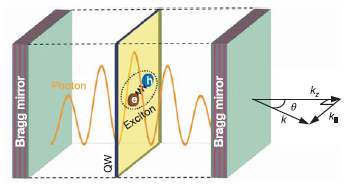
\includegraphics[width=.8\linewidth]{cavity}
  \caption{
    % 
    Pictorial representation of microcavity polaritons, as electron-hole pairs (excitons) inside a semiconductor quantum well (QW), 
    coupled with the photons trapped by the dielectric Bragg mirrors of the cavity. 
    Momentum conservation dictates that a cavity field component of momentum $\kv$ must decay into external radiation of frequency $\omega$, emitted at an angle $\theta$ satisfying $k c = \omega \sin\theta$.
    From Ref.~\cite{Kasprzak_2006}.
    % 
  }\label{fig:cavity-polaritons}
\end{figure}

\subsection{Microscopic description}
\label{subsec:microscopic}


We start by writing down the kinetic energy of the cavity photons
%
\begin{equation}\label{eq:cavity-energy}
  H_{C} = \sum_{\kv} \omega_C(k) a_{\kv}^{\dagger} a_{\kv}
\end{equation}
% 
where we've made use of the translational symmetry of the problem in
the $(x,y)$ plane and labeled the bosonic creation (annihilation)
operators $a_{\kv}^{\dagger}$ ($a_{\kv}$) by the in-plane momentum
$\kv$. These operators satisfy the standard commutation relations
\begin{align}
  \left[a_{\kv}, a_{\kv^{\prime}}^{\dagger}\right] & =\delta_{\kv,\kv^{\prime}}\\
  \left[a_{\kv}, a_{\kv^{\prime}}\right] & =\left[a_{\kv}^{\dagger}, a_{\kv^{\prime}}^{\dagger}\right] = 0
\end{align}

The confinement along the $z$ direction leads to the quantization of
the photon momentum $k_z = \pi N/l_z$, with $N = 1,2,\dots$ indexing
the longitudinal modes. Fig.~\ref{fig:cavity-polaritons} depicts the
photonic field corresponding to the $N = 5$ mode as a standing wave,
representing the measurable electric field inside the cavity. This
field can be expressed in terms of photonic operators by
$E(\kv,z)a_{\kv} +$ H.c., where the photon mode wavefunction
$E(\kv,z)$ has the sinusoidal shape~\cite{Carusotto_2013}
%
\begin{equation}\label{eq:electric-field}
  E(\kv,z) \propto \sqrt{\omega_C(k)/l_z} \sin \left(k_z z\right)
\end{equation}
% 


The cavity photon dispersion for each of these modes is therefore
$\omega_C(k) = v \sqrt{k^2 + k_z^2}$, with $v$ the speed of light in
the semiconductor. Expanding the square root for $k \ll k_z$, one gets
$\omega_C(k) \approx \omega_C(0) + k^2/(2m_{C})$. We see that cavity
photons, as opposed to free-space photons, have a quadratic dispersion
with an effective mass $m_C$ related to the cutoff frequency $\omega_C(0)$
by $m_{C} v^2 = \omega_C(0)$. For typical cavities used in
experiments, $m_{C}$ is of the order of $10^{-5}$ (free) electron
masses $m_e^0$ (see Tab.~\ref{tab:GaAs-params}).

We now turn our attention to the semiconductor QW. For simplicity,
consider a spin-polarized direct bandgap semiconductor such as GaAs,
so that we can neglect additional spin degrees of freedom. We further
assume that the dispersions of single particle states in the
conduction and valence bands have the quadratic form
$\varepsilon^c_{k} = \varepsilon_g/2 + k^2/(2m_e)$ and
$\varepsilon^v_{k} = - \varepsilon_g/2 - k^2/(2m_h)$, with
$\varepsilon_g$ the semiconductor bandgap and $m_e$ and $m_h$ the
effective masses for electrons and (heavy) holes. Excitons have a
typical extension $\lambda_X = \frac{\epsilon}{2\mu e^2}$ called the
(2D) exciton Bohr radius, with $\epsilon$ the static dielectric
constant, $e$ the electron charge and $\mu^{-1} = m_e^{-1} + m_h^{-1}$
their reduced mass. Their binding energy is called the exciton
Rydberg, defined as $\Ry_X = \frac{e^2}{\epsilon \lambda_X}$.

We further define $c_{\kv}^{\dagger}$ and $v_{\kv}$ as the operators which
create an electron in the empty conduction band, respectively a hole
in the filled valence band, and which obey the Fermi anticommutation
rules
\begin{align}
  \left\{c_{\kv}, c_{\kv^{\prime}}^{\dagger}\right\} & =\delta_{\kv,\kv^{\prime}}\\
  \left\{c_{\kv}, c_{\kv^{\prime}}\right\} & = \left\{c_{\kv}^{\dagger}, c_{\kv^{\prime}}^{\dagger}\right\} = 0
\end{align}
and similar for $v_{\kv}$. We can therefore write the electronic
Hamiltonian in terms of these new operators as~\cite{Keeling_2007}
%
\begin{equation}\label{eq:coulomb-hamiltonian}
  H_{\text{el}} = \sum_{\kv} \left( \varepsilon^c_k c_{\kv}^{\dagger} c_{\kv} + \varepsilon^v_k v_{\kv}^{\dagger} v_{\kv} \right) + \frac{1}{2}\sum_{\bm{q}} V_q \left( \rho^e_{\bm{q}} \rho^e_{-\bm{q}} + \rho^h_{\bm{q}} \rho^h_{-\bm{q}} -2 \rho^e_{\bm{q}} \rho^h_{-\bm{q}}\right)
\end{equation}
% 
Here we have introduced the electron and hole densities,
$\rho^e_{\bm{q}} = \sum_{\kv} c_{\kv + \bm{q}}^{\dagger} c_{\kv}$ and
$\rho^h_{\bm{q}} = \sum_{\kv} v_{\kv} v_{\kv + \bm{q}}^{\dagger}$. The
matrix element of the Coulomb potential
$V_q = \frac{e^2}{2 \epsilon A q}$ depends on cavity quantization area
$A$, but this dependence drops out when passing from discrete sums
over states to integrals over the momenta $\kv$.

Finally, the last ingredient of our microscopic description concerns
the interaction between electrons and photons. Making use of the
dipole approximation, we have
%
\begin{equation}\label{eq:dipolar-inter}
  H_{\text{dipole}} = \sum_{\kv, \bm{q}} G(q) \left( a_{\bm{q}}^{\dagger} v_{\kv + \bm{q}}^{\dagger} c_{\kv} + \text{H.c.}\right)
\end{equation}
% 
with the strength
$G(k) = e \mu_{\text{cv}}\sqrt{\frac{\omega_C(k)}{2\epsilon A l_z}}$
written in the dipole gauge, where $\mu_{\text{cv}}$ is the inter-band
dipole matrix element.


\subsection{Effective Hamiltonian}
\label{subsec:effective}


As mentioned in Sec.~\ref{subsec:model}, we are interested in an
approximate description of the problem where we can consider the
excitons as fundamental quasiparticle excitations from the ground
state of the semiconductor and treat the Coulomb term in
Eq.~\eqref{eq:coulomb-hamiltonian} as an effective exciton-exciton
interaction. We then couple the resulting excitons to light, and
obtain the so-called \textit{weakly interacting boson model} for
polaritons. The name stems from the fact that, at moderate
electron-hole densities, such that the inter-exciton distance is much
larger than $\lambda_X$, one can assume excitons to behave esentially
as (composite) bosons~\cite{deveaud2003electron}, and therefore
describe them using the Bose creation and annihilation operators
$b_{\kv}^{\dagger}$ and $b_{\kv}$. Making an Usui
transformation~\cite{Usui1960} and truncating the interaction terms at
fourth order results in the following three-part effective
Hamiltonian~\cite{Ciuti_2003}
%
\begin{equation}\label{eq:total-ham}
  H_{\text{eff}} = H_0  + H_{\text{XX}} + H_{XC}^{\text{sat}}
\end{equation}
% 
where we have defined
\begin{align}
  H_0 & =\sum_{\kv}\left(a_{\kv}^{\dagger},\, b_{\kv}^{\dagger}\right)\mat{\omega_C(k)}{\Omega_R}{\Omega_R}{\omega_X(k)}\colvec{a_{\kv}}{b_{\kv}}\label{eq:polariton-ham}\\
  H_{\text{XX}} & =\frac{1}{2}\sum_{\kv,\kv^{\prime},\bm{q}}U_{\kv - \kv^{\prime},\bm{q}}b_{\kv + \bm{q}}^{\dagger}b_{\kv^{\prime} - \bm{q}}^{\dagger}b_{\kv^{\prime}}b_{\kv}\label{eq:interaction-ham}\\
  H_{XC}^{\text{sat}} & =-\frac{\Omega_R}{\rho_{\text{sat}}A}\sum_{\kv,\kv^{\prime},\bm{q}}\left(b_{\kv^{\prime}-\bm{q}}^{\dagger}b_{\kv + \bm{q}}^{\dagger}b_{\kv}a_{\kv^{\prime}} + \text{H.c.}\right)\label{eq:saturation-ham}
\end{align}
$H_0$ contains the kinetic energy of the excitons and cavity photons,
as well as their harmonic coupling, ie. the conversion of an exciton
to a cavity photon at the Rabi frequency $\Omega_R$, which depends on
the overlap between the wavefunctions of the exciton and photon
through the  oscillator strength surface density $f_{\text{2D}}$ of
the excitonic transition
%
\begin{equation}\label{eq:omega-R}
  \Omega_R \propto \frac{E(z_{\text{QW}})}{E_{\text{max}}}\sqrt{f_{\text{2D}}\omega_C(0)/l_z}
\end{equation}
% 
where $E_{\text{max}}$ is the maximum amplitude of the cavity photon
electric field, at one of its antinodes from
Eq.~\eqref{eq:electric-field}. It is worth noting that both
Eq.~\eqref{eq:dipolar-inter} and Eq.~\eqref{eq:polariton-ham} make use
of the rotating-wave approximation, neglecting antiresonant terms
which do not conserve the number of excitations, such as
$b_{\kv}a_{\kv}$ and $b_{\kv}^{\dagger}a_{\kv}^{\dagger}$. This is
justified so long as $\Omega_R \ll \omega_C(0),\, \omega_X(0)$, which
is normally the case, as can be seen by inspecting
Tab.~\ref{tab:GaAs-params}.

Eq.~\eqref{eq:polariton-ham} can be diagonalized by means of a unitary
transformation of the form~\cite{Hopfield1958}
%
\begin{equation}\label{eq:hopfield-trans}
  \colvec{p_{\kv}}{u_{\kv}} = \mat{X_k}{C_k}{-C_k}{X_k} \colvec{b_{\kv}}{a_{\kv}}
\end{equation}
% 
The normal modes of $H_0$ are called \textit{upper and lower
  polaritons} (UP and LP) and correspond to the Bose operators
$u_{\kv}$ and $p_{\kv}$, with eigenenergies
%
\begin{figure}[tb]\centering
  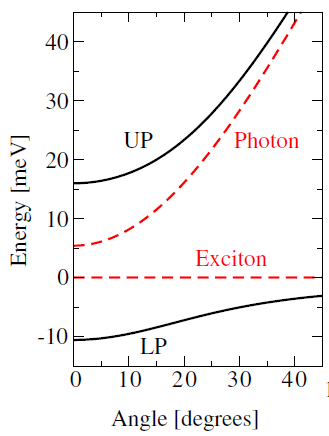
\includegraphics[width=.5\linewidth]{polariton_dispersion}
  \caption{
    % 
    Dispersion relation for the two polaritonic branches (UP, LP) as a function of emission angle $\theta$ of photons outside the cavity, which is directly related to the momentum $\kv$ of polaritons inside the cavity. The exciton and cavity photon dispersions are depicted with dashed (red) lines. Due to their light mass, the polaritons have a very sharp dispersion  compared to excitons. Also note the typical anticrossing form characteristic of Hermitian coupling.
From Ref.~\cite{Keeling_2007}.
    % 
}\label{fig:polariton-dispersion}
\end{figure}
% 
\begin{equation}\label{eq:polariton-dispersion}
  \omega_{\text{UP,LP}}(k) = \frac{1}{2}\left(\omega_C(k) + \omega_X(k)\right) \pm \frac{1}{2}\left[\left(\omega_C(k) - \omega_X(k)\right)^2 + 4 \Omega_R^2\right]^{1/2}
\end{equation}
% 
where the $\pm$ signs refer to the UP and LP branches and the Hopfield
coefficients appearing in Eq.~\eqref{eq:hopfield-trans} are
\begin{align}
  X_k & =\left[1 + \left(\frac{\Omega_R}{\omega_{\text{LP}}(k) - \omega_C(k)}\right)^2\right]^{-1/2}\label{eq:hopfield-X}\\
  C_k & =-\left[1 + \left(\frac{\omega_{\text{LP}}(k) - \omega_C(k)}{\Omega_R}\right)^2\right]^{-1/2}
\end{align}
The two branches of the polaritonic dispersion relation are shown in
Fig.~\ref{fig:polariton-dispersion}, together with the dispersions of
the cavity photons and excitons. One can therefore think of polaritons
as being massive photons dressed by matter excitations.

Note that the 1s-exciton energy can be approximated as
$\omega_X(k) = \omega_X(0) + \frac{k^2}{2M}$, with the exciton mass
$M = m_e + m_h$ of the order of the electron mass and
$\omega_X(0) = \varepsilon_g - \Ry_X$. Since, as we have already
noted, $M$ is several orders of magnitude larger than the cavity
photon mass $m_{C}$, one can in practice neglect the momentum
dependence of the excitonic dispersion, considering it as
flat. Furthermore, we can agree to measure energies starting from
$\omega_X(0)$ and denote the detuning between exciton and photon bands
as $\delta \equiv \omega_C(0) - \omega_X(0)$. For zero detuning
($\delta = 0$), the splitting between the two polariton branches is
$2\Omega_R$. In order to tune $\delta$ in experiments, one tipically
builds the cavity mirrors with a wedge~\cite{Weisbuch1992}.



$H_{\text{XX}}$ quantifies the effective repulsive exciton-exciton
interaction, with a momentum dependent strength
$U_{\kv - \kv^{\prime},\bm{q}}$ that can be calculated from the
Coulomb exchange term in the Born approximation.  Notice that the
form of this interaction corresponds to Feynman diagrams with
4-legged vertices in quantum field theory language, implying binary
collision with momentum conservation: two excitons in the planewave
states $\ket{\kv}$ and $\ket{\kv^{\prime}}$ scatter into the new
states $\ket{\bm{\kv+\bm{q}}}$ and $\ket{\bm{\kv^{\prime}-\bm{q}}}$.
A further approximation that one can make for wave vectors much
smaller than $\lambda_X^{-1}$ is to reduce
$U_{\kv - \kv^{\prime},\bm{q}}$ to a contact potential
$g_X \equiv \frac{1}{2} U_{\bm{0},\bm{0}} =
\frac{6e^2\lambda_X}{2A\epsilon}$, as shown in
Ref.~\cite{Ciuti1998}. As a result, $g_X$ physically represents the
interaction between two excitons in the same single-particle momentum
eigenstate $\ket{\kv}$.

Finally, the last term of Eq.~\eqref{eq:total-ham},
$H_{\text{XC}}^{\text{sat}}$, can be interpreted as a saturation
effect due to the Pauli exclusion principle underlying the fermionic
character of the excitons~\cite{Tassone1999}. The exciton saturation
density $\rho_{\text{sat}} \sim \frac{7}{16\pi\lambda_X^2}$ generally
depends on the specific shape of the internal wavefunction of the
exciton~\cite{Glazov2009}.  For the problems we will be treating in
the remainder of this manuscript it can be considered large enough to
justify neglecting this anharmonic contribution to the total
Hamiltonian Eq.~\eqref{eq:total-ham} (see Tab.~\ref{tab:GaAs-params}).

Before concluding this Section, one should mention the validity
limitations of the weakly interacting boson model for polaritons
reviewed here. Its derivation, by means of the Usui transformation,
implies an expansion of the original fermionic operators of
Eq.~\eqref{eq:coulomb-hamiltonian} in powers of bosonic operators,
having as small parameter the number of excitons per Bohr radius
$\lambda_X$. Truncating this series at fourth order results in an
upper bound on the exciton density of around $1/\lambda_X^2$. At
higher densities, an electron-hole plasma-like state is formed, with a
a qualitatively different behaviour~\cite{COMBESCOT2008}.  We see that
this model is particularly useful for the case when the dominant
interaction is the Coulomb repulsion between the excitons.

\subsection{Lower polaritons}
\label{subsec:lower-polaritons}

Assuming the Rabi energy $\Omega_R$ to dominate over the kinetic and
interaction energies we can neglect the upper polaritons and project
Eq.~\eqref{eq:total-ham} on the basis of lower-polariton states
only. Employing the approximations discussed above, we obtain the
lower-polariton Hamiltonian
%
\begin{equation}\label{eq:LP-ham}
  H_{\text{LP}} = \sum_{\kv} \omega_{\text{LP}}(k) p_{\kv}^{\dagger} p_{\kv} + \sum_{\kv,\kv^{\prime},\bm{q}} V^{\text{eff}}_{\kv,\kv^{\prime},\bm{q}}\, p^{\dagger}_{\kv + \bm{q}} p^{\dagger}_{\kv^{\prime} - \bm{q}} p_{\kv} p_{\kv^{\prime}}
\end{equation}
% 
where the strength of the repulsive interaction between lower
polaritons now depends on in-plane momentum through the Hopfield
coefficients\footnote{The interaction strength $g_X$ can usually be
  rescaled to 1 by a simple transformation.}
%
\begin{equation}\label{eq:g-eff}
  V^{\text{eff}}_{\kv,\kv^{\prime},\bm{q}} = g_X X_{\kv + \bm{q}}X_{\kv^{\prime} - \bm{q}}X_{\kv}X_{\kv^{\prime}}
\end{equation}
% 
This effective interaction, originating from the binary Coulomb
scattering of the excitons, is the one responsible for the collective
behaviour of the polaritons, and in particular superfluid
hydrodynamics, an aspect which we will explore in the following two Chapters.

Physically, the quantities $\abs{X_k}^2$ and $\abs{C_k}^2$ are the
excitonic and photonic fractions of the lower polariton mode and the
effective mass of the lower polaritons, $m_{\text{LP}}$, can be
computed from the curvature of their dispersion
Eq.~\eqref{eq:polariton-dispersion} by
%
\begin{equation}\label{eq:LP-mass-def}
  m_{\text{LP}}(k) = \left[\frac{d^2 \omega_{\text{LP}}(k)}{dk^2}\right]^{-1}
\end{equation}
% 
which at normal incidence $\kv = 0$ reduces to 
%
\begin{equation}\label{eq:LP-mass}
  m_{\text{LP}} = 2m_C \left[1 - \delta/\sqrt{\delta^2 + 4\Omega_R^2}\right]^{-1}
\end{equation}
% 
if we neglect the flat exciton dispersion in the limit $M \gg
m_C$. For zero detuning, we see that $m_{\text{LP}} = 2m_C$ and the
light and matter content of lower polaritons are each equal to $1/2$.

As long as the interesting physics is limited to small wavevectors
$\kv$, close to the bottom of the LP branch, one can safely
approximate the LP dispersion as being parabolic, by expanding
Eq.~\eqref{eq:polariton-dispersion} in a Taylor series around
$\kv = 0$ and truncating at second order. We obtain the expression
%
\begin{equation}\label{eq:parabolic-disp}
  \omega_{\text{LP}}(k) \simeq \omega_{\text{LP}}(0) + \frac{k^2}{2m_{\text{LP}}}
\end{equation}
% 
with an effective mass given by Eq.~\eqref{eq:LP-mass}. In practice,
many interesting experimental conditions can be adequately described
by limiting ourselves to the LP branch with a quadratic dispersion.


\subsection{Pumping and dissipation}
\label{subsec:pumping}

We have so far assumed that the mirrors at the two ends of the optical
cavity in Fig.~\ref{fig:cavity-polaritons} are perfect. In reality of
course, this is not the case, and photons continuously escape from the
cavity. In other words, dissipation is a built-in feature of this
system and, rather than being a hindrance, it is actually useful as it
allows one to extract information about the system. By looking at
the near-field (far-field) emission from the cavity, one can measure
the real (momentum) space photon density. The polaritonic spectrum can
also be obtained in this way, as a function of the angle $\theta$ of
emission of a photon out of the cavity, as shown in
Fig.~\ref{fig:polariton-dispersion}.

Since the system is lossy, one needs to drive it by means of an
incoming laser beam (called the pump), thus replenishing the photons
and achieving a stationary state. It is important to note, however,
that this state should not be confused with thermal equilibrium, as we
are dealing with intrinsic out-of-equilibrium physics
here. Experiments have so far explored two main ways of pumping these
cavities: resonantly (coherent) and non-resonantly (incoherent). We
will not concern ourselves with the latter in this manuscript, but we
point the interested reader to the excelent review in
Ref.~\cite{Carusotto_2013} (and references therein) for details.

Resonant pumping is done by means of a continuous-wave coherent laser
beam which is transmitted through one of the mirrors. The coherence of
the beam is then inherited by the polariton fluid.  As already
mentioned, conservation of in-plane momentum and photon frequency
dictates that a laser wave coming in at an angle $\theta$ and
frequency $\omega$ resonantly excites a microcavity mode with
wavevector $k_{\parallel} = \frac{\omega}{c}\sin(\theta)$ (see
Fig.~\ref{fig:cavity-polaritons}). As a result, we see that, besides
balancing the losses, the pump can also be used to tune the system to
a particular desired state, injecting polaritons of a given momentum
and energy. In the following we will consider that the pumping is done
quasi-resonantly, close to the bottom of the LP branch, by using a
homogeneous planewave pump of amplitude $f_p$, wavevector $\kv_p$,
frequency $\omega_p$ and circular polarization
\begin{equation}\label{eq:pwpump}
  \mathcal{F}(\bm{r},t) = f_p \exp{\left[i (\bm{k}_p \cdot \bm{r} -
    \omega_p t)\right]}
\end{equation}

Depending on the pump parameters (specifically the pumping angle,
which in turn determines $k_p$), one can distinguish two qualitatively
different regimes: the pump-only state where where the only stable
configuration of the system is the mode at $k_p$ and the regime where
polaritons at $k_p$ undergo stimulated scattering and populate two
other modes. Indeed, if the pumping angle is such that the wavevector
it excites lies close to the inflection point of the LP dispersion,
the system can enter a new regime called \textit{optical parametric
  oscillator} (see Sec.~\ref{subsec:opo} for details about OPO).

To quantitatively account for the driving and dissipation, one can use
the input-output formalism that was extended to planar microcavities
in Ref.~\cite{Ciuti2006}. As far as photonic losses are concerned, we
must first note that, apart from the radiative decay channels already
mentioned, there is also a nonradiative contribution due to photon
absorbtion inside the cavity. The total cavity photon decay rate
$\gamma_C$ can therefore be expressed as the sum
$\gamma_C^{\text{rad}} + \gamma_C^{\text{nrad}}$, where the radiative
decay rate
%
\begin{equation}\label{eq:rad-decay}
  \gamma_C^{\text{rad}}(\kv) = -2 \eta(\kv)\kappa(\kv)
\end{equation}
% 
is a function of the input (output) coefficients $\eta$ ($\kappa$)
that can generally be computed via the transfer matrix
method~\cite{burstein2012confined}. For the simple case of normal
incidence and mirror transmittivity $t \ll 1$, these coefficients are
given by~\cite{Carusotto_2013}
\begin{align}
  \begin{split}
    \eta(\kv) & =(c t/2l_z) \sqrt{l_z/\pi\omega_C(\kv)}\\
    \kappa(\kv) & =-t\,\sqrt{\pi \omega_C(\kv) / l_z}  
  \end{split}
\end{align}
with $c$ the speed of light in vacuum.

The excitons from the QW are of course also subject to decay
processes. While their radiative decay can only take place via one of
the cavity modes (due to strong light-matter coupling\footnote{In
  general, one is in the strong coupling regime when $\Omega_R$ is
  greater than the combined losses in the system.}), we must include
nonradiative recombination processes as well as the additional
dephasing~\cite{Liew2011} caused by interactions with carriers inside
the well and variations in well thickness. All this results in an
effective decay rate $\gamma_X$ for excitons, which is generally
weaker than the photonic one quantified by $\gamma_C$. Typical values
of both rates for GaAs-based microcavities are shown in
Tab.~\ref{tab:GaAs-params}.


\subsection{Disorder effects}
\label{subsec:disorder}


It is noteworthy to remark that Hamiltonian Eq.~\eqref{eq:total-ham}
does not include any disorder. We have already mentioned that there
are two distinct disorder classes in this problem. One is the
excitonic disorder, acting on length scales of around 10 nanometers,
which tipically affects the exciton oscillator strengths
$f_{\text{2D}}$, but not the spatial polaritonic density. This type of
disorder stems from variations in the QW thickness as well as alloy
imperfections and is typically not strong enough to dissociate
excitons. Neglecting excitonic disorder also implies that each
localized exciton state couples to precisely one extended photon
state. The resulting polaritons are then nothing but the coherent
superposition of these excitonic and photonic states.

Photonic disorder, on the other hand, acts on lengthscales
$\ell_{C} = (m_{C}\Omega_R)^{-1/2}$ on the order of microns (see
Tab.~\ref{tab:GaAs-params}) and therefore can disrupt the polariton
density profile. Photonic disorder is normally caused by the presence
of imperfections inherent to the growth process of the cavity
mirrors. These defects act as scattering centers for the polaritons,
and can be included in the Hamiltonian as an additional external
scalar potential. The simplest example is that of a spatially
localized defect of strength $g_V$ located at positon $\rv_0$, which
can be approximated by the potential
%
\begin{equation}\label{eq:defect-pot}
  \tilde{V}_d(\rv) = g_V \delta^2(\rv - \rv_0)
\end{equation}
% 

\subsection{Realistic systems}
\label{subsec:realistic}

To get a more quantitative idea of the physics involved, it is worth
describing realistic samples typically used in state-of-the-art
experiments. Instead of simple metallic mirrors, such microcavities
are usually bound by a series of up to around 20 distributed Bragg
reflectors (DBRs), which are alternating dielectric layers of
thickness $\lambda/4$ and different refractive indices, achieving a
total reflectivity of over $99.9$\%~\cite{9780199228942}. 

Multiple CdTe or GaAs QWs a few nanometers thick are placed inside the
cavity of length $l_z = 2\lambda \sim 1~\mu$m, at the antinodes
(maxima) of the photonic electric field, in order to maximize the
coupling between excitons and photons (see Eq.~\eqref{eq:omega-R},
which shows maximum coupling for $E(z_{\text{QW}}) =
E_{\text{max}}$). When $N$ distinct QWs are placed in the cavity at
the electric field maxima, the light-matter coupling $\Omega_R$ is
enhanced by a factor $\sqrt{N}$. Furthermore, the cavity cutoff
frequency $\omega_C(0)$ is normally chosen close to the exciton
frequency $\omega_X(0)$.

Typical values of the relevant parameters for GaAs-based
microcavities are shown in Tab.~\ref{tab:GaAs-params}. 
%
\begin{table}
  \centering
  \begin{tabular}{@{}ll@{}} \toprule
    QW & Cavity \\ \midrule
    $\epsilon \simeq 13$ &  $\omega_C(0) \simeq \omega_X(0) \simeq 1.53$~eV\\
    $m_e = 0.063m^0_e$    &  $\delta \in [-10,10]$~meV\\
    $m_h = 0.3m^0_e$      &  $m_{C} = 2.3\times 10^{-5} m^0_e$ \\
    $\lambda_X \simeq 7$~nm   & $\ell_{C} = 0.868~\mu$m\\
    $\Ry_X \simeq 17$~meV &  $\Omega_R \simeq 2.2$~meV \\
    $\gamma_X \sim \mu$eV &  $\gamma_C = 0.1$~meV \\ 
    $g_X \simeq 5\times10^{-3}$~meV($\mu$m)$^2$ &  $A \sim 10^4~\mu$m$^2$\\
    $\rho_{\text{sat}} \simeq 2842~$($\mu$m)$^{-2}$ &  $l_z \sim 1~\mu$m\\ \bottomrule
  \end{tabular}
  \caption{Typical parameters of a microcavity containing GaAs QWs. Left column shows properties of the QW, while the right one refers to the microcavity. For these values, the ratio between saturation and
    Coulomb interaction is small,
    $\Omega_R/(g_X \rho_{\text{sat}}) \simeq 0.1$. From Ref.~\cite{9783642241857}.}
  \label{tab:GaAs-params}
\end{table}
%


\subsection{Mean-field description}
\label{subsec:mean-field}

As it turns out, a useful approach for tackling the
hydrodynamics-related problems that we will encounter in the following
Chapters is the so-called mean-field approximation. In the context of
weakly interacting Bose gases, this approach leads to the celebrated
Gross-Pitaevskii equation~\cite{9780198507192}, and in our case it
will lead to its driven-dissipative counterpart.

If the Rabi energy is larger than the pump detuning from the bottom of
the LP branch $\omega_p - \omega_{\text{LP}}(0)$ and also larger than
the decay rates $\gamma_X$ and $\gamma_C$, we can start from the lower
polariton Hamiltonian of Sec.~\ref{subsec:lower-polaritons}.  The idea
is that one replaces the lower polariton operators $p_{\kv}$ in
Eq.~\eqref{eq:LP-ham} with their expectation values
$\psi_{\kv} = \langle p_{\kv} \rangle$, where $\psi_{\kv}$ is now
interpreted as a classical field (order parameter representing lower
polariton polarization) describing the state with momentum label
$\kv$. The mean-field equation for $\psi_{\kv}$ is then obtained from
the Heisenberg equation of motion
$\dot{p}_{\kv} =i \left[ H_{\text{LP}},\, p_{\kv} \right]$ by
replacing all the operators with their corresponding expectation
values. This mean-field treatment is of course exact as far as the
pumping and the losses are concerned, as well as for any two-operator
product such as the polariton kinetic energy. However, the effective
lower polariton interactions are approximated following an approach
similar to the one pioneered by Bogoliubov in the context of atomic
BECs, namely
%
\begin{equation}\label{eq:mean-field-approx}
  \langle p^{\dagger}_{\kv_1 + \kv_2 - \kv} p_{\kv_2} p_{\kv_1} \rangle \approx \langle p_{\kv_1 + \kv_2 - \kv} \rangle^{\star} \langle p_{\kv_2} \rangle \langle p_{\kv_1} \rangle
\end{equation}
% 
We obtain a generalized Gross-Pitaevskii equation (GPE) in momentum
space under coherent driving, which includes losses and describes the
time evolution of $\psi_{\kv}(t)$
%
\begin{multline}\label{eq:mom-GPE}
  i\partial_t\psi_{\kv} = \left[\omega_{\text{LP}}(k) - \frac{i}{2} \gamma_k\right]\psi_{\kv} + \sum_{\kv_1,\kv_2} g_{\kv,\kv_1,\kv_2} \psi^{\star}_{\kv_1 + \kv_2 - \kv} \psi_{\kv_2} \psi_{\kv_1}\\
  + C_{\kv} \sum_{\bm{q}} C_{\bm{q}} V_d(\kv - \bm{q}) \psi_{\bm{q}}
  + C_{\kv} f_p \exp{\left(-i \omega_pt\right)} \delta_{\kv,\kv_{p}}
\end{multline}
Here $\gamma_k = \gamma_X \abs{X_k}^2 + \gamma_C \abs{C_k}^2$ is the
(lower) polariton loss rate, $V_d(\kv)$ is the Fourier transform of
the external potential Eq.~\eqref{eq:defect-pot} and the effective
polariton-polariton interaction strength is given by
%
\begin{equation}\label{eq:LP-inter}
  g_{\kv,\kv_1,\kv_2} = g_X X_{\kv}X_{\vert\kv_1 + \kv_2 - \kv\vert}X_{\kv_1}X_{\kv_2}
\end{equation}

Going beyond the mean-field approximation to include quantum and
thermal fluctuations of the (quantum) field $\hat{\psi}_{\kv}$ is not
an easy task in general, see Ref.~\cite{Carusotto_2013} for some
approaches such as using the semiclassical Wigner representation.


In order to obtain the corresponding form of Eq.~\eqref{eq:mom-GPE} in
real-space, we introduce the Fourier transform of the classical
wavefunction $\psi_{\kv}$ by means of\footnote{Replacing the discrete
  sums over $\kv$ states by continuous integrals is justified in the
  limit of a large system.}
%
\begin{equation}\label{eq:fourier-psi}
  \tilde{\psi}(\rv) = \int \frac{d^2\kv}{(2\pi)^2} \psi(\kv) \exp \left(i \kv \cdot\rv \right)
\end{equation}
% 
Knowing that Fourier transforms take multiplication to convolution, we
immediately get the real-space equation for $\tilde{\psi}(\rv, t)$
\begin{multline}\label{eq:convoluted-GPE}
  i \partial_t \tilde{\psi}(\rv) = \left[ \omega_{\text{LP}}(-i \bm{\nabla}) - \frac{i}{2} \gamma(-i \bm{\nabla}) \right] \tilde{\psi}(\rv)\\ + \int d\rv_{1,2,3} \,\tilde{g}(\rv_1 - \rv, \rv - \rv_2, \rv - \rv_3) \tilde{\psi}^{\star}(\rv_1) \tilde{\psi}(\rv_2) \tilde{\psi}(\rv_3)\\
+ \int d\rv_{1,2} \,\tilde{C}(\rv - \rv_1) \tilde{C}(\rv_1 - \rv_2) \tilde{V}_d(\rv_1) \tilde{\psi}(\rv_2) + C(\kv_p) \mathcal{F}(\bm{r},t)
\end{multline}
Note that the kinetic energy operator has a particular dependence on
the gradient instead of the usual Laplacian, reflecting the
non-parabolic LP dispersion.  Furthermore, the nonlocal interaction
term in the second line of Eq.~\eqref{eq:convoluted-GPE} has the form
of the most general third order nonlinear term that one can come up
with, if $\tilde{g}$ were an arbitrary function. This freedom is
somewhat restrained in practice by the fact that $\tilde{g}$ is related to
Eq.~\eqref{eq:LP-inter} by
%
\begin{equation}\label{eq:convoluted-g}
  \tilde{g}(\rv_1, \rv_2, \rv_3) = \int d\kv_{1,2,3} \,g(\kv_1,\kv_2,\kv_3) \exp \left[i \textstyle{\sum_{n=1}^3} (\kv_n \cdot \rv_n) \right]
\end{equation}
% 
and we have also introduced the functions $\tilde{C}(\rv)$, which are
the Fourier transforms of the Hopfield coefficients $C(\kv)$. These
coefficients do not have a very pronounced momentum dependence, as in
fact for $\delta = 0$, $X(\kv)$ is between $1/\sqrt{2}$ and $1$. If we
neglect altogether the Hopfield coefficients in
Eq.~\eqref{eq:convoluted-GPE} and consider the case of parabolic lower
polariton dispersion, we finally obtain the real-space
driven-dissipative GPE in its simplified form
%
\begin{equation}\label{eq:rspace-GPE}
  i \partial_t \tilde{\psi}(\rv) = \left[ \omega_{\text{LP}}(0) - \frac{\nabla^2}{2m_{\text{LP}}} - \frac{i}{2}\gamma  + \tilde{V}_d(\rv) + g_X \abs{\tilde{\psi}(\rv)}^2\right] \tilde{\psi}(\rv)
  + \mathcal{F}(\bm{r},t)
\end{equation}
% 
Here we have also neglected the momentum dependence of the polariton
loss rate, justified by the fact that, at large momenta, the
diminishing radiative width is normally compensated by non-radiative
broadening.  To make a stronger connection with nonlinear optics, we
note that a similar equation holds for cavities containing a nonlinear
medium, with the role of $g_X$ being taken by the $\chi^{(3)}$
susceptibility of the medium~\cite{boyd2003nonlinear}. This equation
allows for an ab-initio description of the coherently pumped system,
unlike the more complicated case of incoherent pumping where one
generally also needs a phenomenological description of the various
relaxation processes~\cite{Keeling_2007}.



\subsection{Equation of state}
\label{subsec:eq-state}

Given that we drive the system with the coherent continuous-wave pump Eq.~\eqref{eq:pwpump}, we can look for stationary state solutions with similar oscillatory behaviour, namely
%
\begin{equation}\label{eq:pump-ansatz}
  \psi(\rv,t) = \psi_p e^{i (\kv_p \cdot \rv- \omega_p t)}
\end{equation}
% 
Inserting this ansatz into Eq.~\eqref{eq:mom-GPE} (without the defect
potential term), we obtain the equation of state for lower polaritons,
employing the simplified notation $\gamma_p \equiv \gamma(\kv_p)$,
$C_p \equiv C(\kv_p)$, $X_p \equiv X(\kv_p)$ and
$\omega^p_{\text{LP}} \equiv \omega_{\text{LP}}(\kv_p)$
%
\begin{equation}\label{eq:pump-mf}
  \left[ \omega_p - \omega^p_{\text{LP}} - g_X X_p^4 \abs{\psi_p}^2 + \frac{i}{2}\gamma_p\right]\psi_p = C_p f_p
\end{equation}
% 
One immediately notices that, unlike the case of the atomic mean-field
Eq.~\eqref{eq:atom-MF}, the phase of the polariton field amplitude
$\psi_p$ is set by the pump, therefore explicitly breaking the $U(1)$
gauge symmetry associated with global rotations of the condensate
phase. This implies that, unlike the atomic BECs, no Goldstone branch
will be present in the polaritonic excitation spectrum. Note also that
the oscillation frequency of the condensate wavefunction is fixed by
the pump frequency $\omega_p$. In Chapter~\ref{cha:drag}, we will
compare the main features of the quasiparticle excitation spectrum for
polaritons to equilibrium systems like cold atomic gases in the BEC
regime.
Another important consequence of this phase-locking is that experiments concerning
topological phase defects such as vortices and solitons should be
performed with a finite size pump, leaving the condensate phase
unbound outside of the pump spot. 
%
\begin{figure}[tb]\centering
  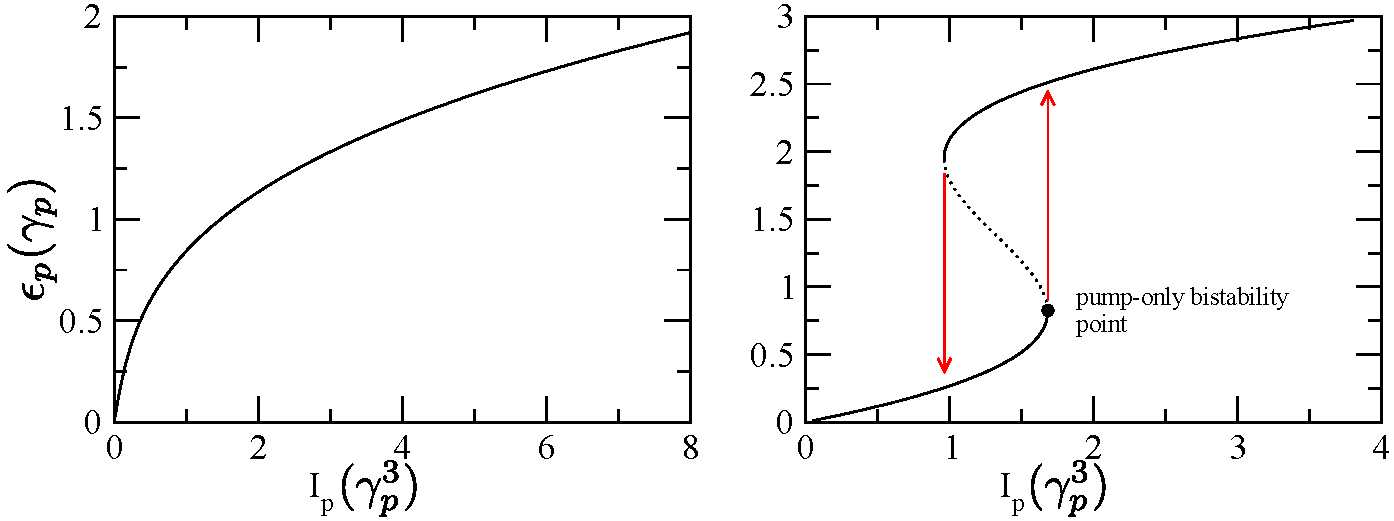
\includegraphics[width=.9\linewidth]{bistable}
  \caption{
    % 
    Pump energy blueshift of Eq.~\eqref{eq:pump-mf-sq} as a function of pump laser intensity in the optical limiter (left panel) and bistable (right panel) regimes. The arrows in the right panel show the hysteretic jumps between the lower and upper branches at different intensities, while the dotted middle branch is single-mode unstable. The black dot marks a saddle node bifurcation. From Ref.~\cite{Wouters_2007_b}.
    % 
  }\label{fig:bistable}
\end{figure}
%

The repulsive polaritonic interaction is responsible for a blueshift
of the LP dispersion $\omega_{\text{LP}}^{p}$.  Introducing the pump energy blueshift
$\epsilon_p = g_X X_p^2 \abs{\psi_p}^2$, we can rewrite
Eq.~\eqref{eq:pump-mf} in absolute value as
%
\begin{equation}\label{eq:pump-mf-sq}
  \left[\left(\frac{\omega_p-\omega^p_{\text{LP}}}{\gamma_p} - X_p^2 \frac{\epsilon_p}{\gamma_p}\right)^2 + \frac{1}{4} \right] \frac{\epsilon_p}{\gamma_p} = X_p^4 \frac{I_p}{\gamma_p^3}
\end{equation}
%
where we have also defined the pump laser intensity
$I_p = g_X C_p^2 \abs{f_p}^2/X_p^2$. One can now distinguish two
qualitatively different regimes, based on the value of the bare pump
detuning $\omega_p-\omega^p_{\text{LP}}$. The first regime, called
\textit{optical limiter} is for
$\omega_p-\omega^p_{\text{LP}} \leq \sqrt{3}\gamma_p/2$ and it is
plotted in the left panel of Fig.~\ref{fig:bistable}. We see that the
pump blueshift increases monotonically with increasing pump power. The
increase is sublinear, as the blueshift moves the lower polariton
dispersion out of resonance with the pump.

The second regime
$\omega_p-\omega^p_{\text{LP}} > \sqrt{3}\gamma_p/2$, shown in the
right panel of Fig.~\ref{fig:bistable}, is called \textit{optical
  bistability} and is no longer monotonic. The blueshift-intensity
curve has a characteric S-shape, and shows hysteresis: increasing the
pump power, we get to the first turning point (filled circle in the
figure) where the blueshift suddenly jumps from the low to the high
branch, while the reverse process of decreasing the pump power shows a
jump at a second turning point on the S curve. Defining an
interaction-renormalized pump detuning
$\Delta_p \equiv \omega_p-(\omega^p_{\text{LP}} + X_p^2\epsilon_p)$,
we see that this quantity is positive up to the second turning point
on the S curve, and then changes sign, becoming negative on the higher
branch.

The middle branch of the S curve, with negative slope, is dynamically
unstable, while the two turning points where the stable and unstable
solutions meet are called \textit{saddle node} bifurcations.  To see
this, one must consider small perturbations of wave-vector $\kv$ of
the form
%
\begin{equation}\label{eq:pump-fluctuations}
  \delta \psi(\rv,t) =  u_p e^{i [(\kv_p + \delta\kv) \cdot \rv - (\omega_p + \omega) t ]}  + v_p^{\star}e^{i[ (\kv_p - \delta\kv) \cdot \rv- (\omega_p - \omega) t]}
\end{equation}
% 
where $\delta\kv \equiv \kv - \kv_p$. Substituting this into
Eq.~\eqref{eq:mom-GPE} and linearising with respect to the amplitudes
$u_p$ and $v_p$, we obtain an eigenvalue problem from which the two
(complex) eigenvalues $\omega$ can be determined in a straightforward
manner. 

Dynamical stability is then ensured iff
$\Im\left[\omega(\kv)\right] < 0$ for all wave-vectors $\kv$.  We can
therefore distinguish two main types of instabilities, depending on
the value of $\delta\kv$: for $\delta\kv =0$ (the degenerate case),
the system shows a \textit{Kerr single-mode} (or pump-only)
instability which only involves the pump wave-vector, while the
general case of $\delta\kv \neq 0$ implies a \textit{parametric}
instability, signaling the onset of the optical parametric oscillator
(OPO) regime. This regime involves two separate modes (apart from the
pump), namely the so-called \textit{signal} and \textit{idler} states
at wavevectors $\kv_s = \kv$ and $\kv_i = 2\kv_p - \kv$ respectively,
as we will discuss at large in Sec.~\ref{subsec:opo}.



\subsection{OPO}
\label{subsec:opo}

To understand why the OPO regime arises, one has to first look at the
form of the Heisenberg equation of motion Eq.~\eqref{eq:mom-GPE}. This
equation describes the coupled dynamics of an arbitrary state $\kv$,
given an applied optical field which excites polaritons with in-plane
wavevector $\kv_p$. As a result of polariton-polariton interactions,
the coherent occupation at generic wavevectors $\kv_1$ and $\kv_2$ can
scatter into $\kv$ and $\kv_1 + \kv_2 - \kv$, a process one can
represent as
%
\begin{equation}\label{eq:scattering-cascade}
  \left\{\kv_1, \kv_2\right\} \rightarrow \left\{\kv, \kv_1 + \kv_2 - \kv\right\}
\end{equation}
% 
As these states further scatter into others by the same matter
wave-mixing mechanism, we get a cascade of so-called satellite states,
with diminishing population.  

Out of the multitude of possible scattering channels, we limit our
description to the one describing the process
$\{\kv_p, \kv_p\} \rightarrow \{\kv, 2\kv_p - \kv\}$, which is
precisely the parametric scattering of two pump polaritons into the
signal and idler states that we just introduced in
Sec.~\ref{subsec:eq-state}. As it turns out, due to the peculiar shape
of the lower polariton dispersion relation
Eq.~\eqref{eq:polariton-dispersion}, this scattering process can occur
in a completely resonant way, with conservation of both in-plane
momentum as well as energy, expressed by the phase-matching conditions
$2\kv_p = \kv_s + \kv_i$ and $2\omega_p = \omega_s + \omega_i$ (we
have introduced here the signal and idler frequencies). The parametric
scattering condition that has to be satisfied then reads
%
\begin{equation}\label{eq:conservations}
  2\omega_{\text{LP}}(\kv_p) =   \omega_{\text{LP}}(\kv_s) +   \omega_{\text{LP}}(\kv_i)
\end{equation}
% 
We must further emphasize the importance of the unique form of the LP
dispersion in Eq.~\eqref{eq:conservations}, as it allows efficient
parametric coupling on a relatively broad range of pump momenta.
Parametric scattering would not be possible for particles with a
quadratic dispersion: in the atomic case for instance, one must employ
the use of an optical lattice in order to deform the dispersion and
promote parametric amplification~\cite{Campbell2006}. 

A schematic depiction of the parametric scattering process with the
signal state located at zero momentum and the pump close to the
inflection point of the LP dispersion is shown in
Fig.~\ref{fig:parametric-scattering}. It is clear that for a given
signal wavevector, Eq.~\eqref{eq:conservations} then uniquely determines
the pump and idler states.
%
\begin{figure}[tb]\centering
  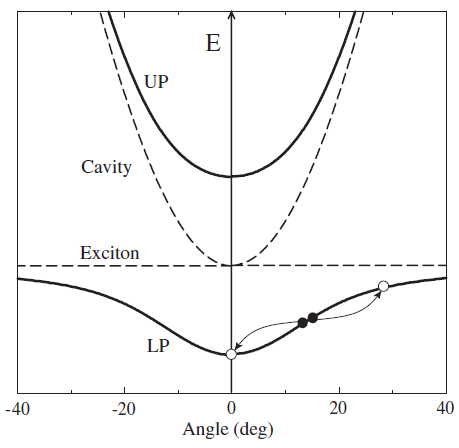
\includegraphics[width=.5\linewidth]{opo}
  \caption{
    % 
    Upper (UP) and lower (LP) polariton dispersions are shown as solid lines, while the original exciton and cavity photon are represented by dashed lines, as a function of the laser incidence angle $\theta$. The filled circles represent two pump polaritons being parametrically scattered into the signal (here at 0 angle) and idler states, shown as empty circles. The scattering process depicted by the curved arrows is resonant, conserving both energy and momentum. From Ref.~\cite{Ciuti_2003}.
    % 
  }\label{fig:parametric-scattering}
\end{figure}
%
The fact that $\kv_s$ is close to $0$ is not incidental, but was
observed in multiple experiments~\cite{Stevenson2000,Baumberg2000}
performed in the OPO regime, as well as numerical simulations of the
full GP equation~\cite{9783642241857}. An intuitive explanation was
put forward~\cite{Gippius2004,Whittaker_2005}, based on the
interaction-induced blueshift of the LP dispersion.

We now turn our attention to the mechanism explaining the onset of the
parametric scattering instability in the simple case of the optical
limiter regime shown in the left panel of Fig.~\ref{fig:bistable}. As
already mentioned, the polariton-polariton repulsive interaction
causes a blueshift of the LP dispersion proportional to the pump mode
population $\abs{\psi_p}^2$. This shift also affects the signal and
idler frequencies $\omega_{\text{LP}}(\kv_{s,i})$, bringing them in
resonance with the pump frequency $\omega_p$. The pump population (and
hence the shift) of the optical limiter is a monotonically increasing
function of laser intensity, quantified by
Eq.~\eqref{eq:pump-mf-sq}. As a result, there is a certain minimum
\textit{threshold intensity} where the resonance starts and the
pump-only solution becomes unstable towards parametric
scattering. Further increasing the laser power, we hit an upper
threshold, where the blueshift becomes too large and the resonance is
lost, forbiding parametric oscillation. This mechanism defines a
certain window of pump intensities where the parametric instability
can arise, the region depicted by the dashed line in
Fig.~\ref{fig:spi}. Inside this window, the pump-only solution still
exists, but it is unstable towards OPO.
%
\begin{figure}[tb]\centering
  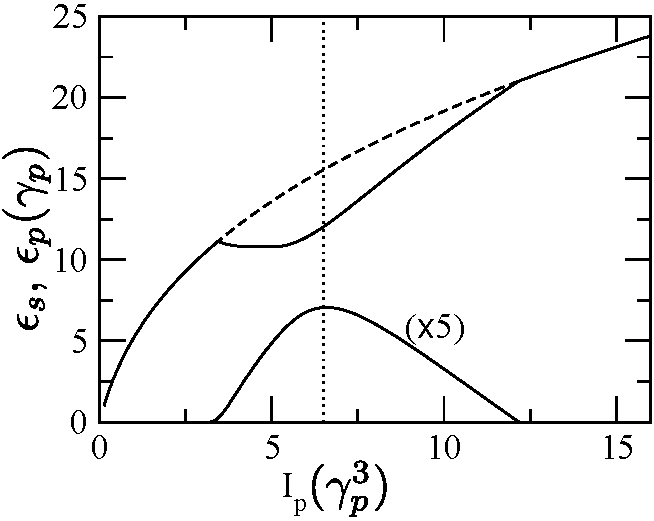
\includegraphics[width=.5\linewidth]{response-sp}
  \caption{
    % 
    OPO pump (upper solid curve) and signal (lower curve, magnified 5 times) energy blueshifts in the optical limiter regime, as a function of pump laser intensity. The dashed line is the pump blueshift in the pump-only solution Eq.~\eqref{eq:pump-mf-sq}. The vertical dotted line marks the pump intensity used in Fig.~\ref{fig:goldstone}.
    From Ref.~\cite{Wouters_2007}.
    % 
  }\label{fig:spi}
\end{figure}
% 

The simplest ansatz one can make for describing the OPO regime above
threshold is to consider the three separate states (signal, pump and
idler), each with its own population, wavevector and frequency, in the
form~\cite{Ciuti_2000,Whittaker2001,Whittaker_2005,Gippius2004}
%
\begin{equation}\label{eq:3-state-ansatz}
  \psi(\rv,t) = \psi_s e^{i (\kv_s \cdot \rv- \omega_s t)} + \psi_p e^{i (\kv_p \cdot \rv- \omega_p t)} + \psi_i e^{i (\kv_i \cdot \rv- \omega_i t)}
\end{equation}
% 
where energy and momentum conservation dictate that
$\omega_i = 2\omega_p - \omega_s$ and $\kv_i = 2\kv_p - \kv_s$. As
before, we insert this ansatz into Eq.~\eqref{eq:mom-GPE} and we
obtain three couplex (complex) equations of motion for $\psi_{s,p,i}$
which determine the dynamics of the signal, pump and idler. It is
important to note that these equations become closed only if we
neglect the multiple scattering processes mentioned at the start of
this Section and consider only the conversion of two pump polaritons
into a signal and an idler polariton. We will not give the full form
of these OPO equations of state, but instead refer the reader to
Ref.~\cite{Wouters_2007_b}, where a complete discussion of the
oscillation threshold and ensuing dynamics is
given. Fig.~\ref{fig:spi} shows a particular solution of the equations
for the optical limiter case. One can see the smooth growth of the
signal population (and subsequent depletion of the pump) inside the
OPO (dashed) region. It is of course never implied that the whole OPO
window is dynamically stable, and in fact a stability analysis needs
to be performed by adding small fluctuations on top of the (now) three
coupled states, in a manner similar to
Eq.~\eqref{eq:pump-fluctuations}, following
Ref.~\cite{Wouters_2007}. The complete treatment will be presented in
Chapter~\ref{cha:opo}.  

Before moving on, it is worth noting that a limitation of the ansatz
Eq.~\eqref{eq:3-state-ansatz} is that it does not allow solving the
so-called ``selection'' problem of determining the value of $\kv_s$
above threshold. As a result, this value has to be considered as an
input parameter to our problem. Futhermore, similarly to the pump-only
case and inherent in any mean-field approach, we are of course
neglecting any quantum fluctuations of the three macroscopically
occupied modes. Last but not least, we are also neglecting the
so-called TE-TM (transverse electric - transverse magnetic)
splitting~\cite{Panzarini1999}, which can act as an effective
spin-orbit interaction term~\cite{Kavokin2004}. This approximation
allows one to work with a single spin state, considering the circular
polarization of the pump to be fully transmitted to the signal and
ider as well.

We now turn our attention to a separate discussion, concerning the
phases of the three OPO states.  As before, the phase of the pump is
fixed by the outside laser, and now the sum of the signal and idler
phases is given by the matching condition
$\phi_s + \phi_i = 2 \phi_p$. Their phase difference however is a
free parameter, and as such it is spontaneously chosen by the system
every time the threshold is crossed. In summary, the OPO equations of
motion for the three states posess a $U(1)$ symmetry, corresponding to
a simultaneous and opposite phase rotation of the signal and idler,
that is
%
\begin{align}
  \begin{split}
    \psi_s& \rightarrow \psi_s e^{i \phi} \\
    \psi_i & \rightarrow \psi_i e^{-i \phi}
  \end{split}
\end{align}
%
This intrinsic symmetry is spontaneously broken above threshold, a
random value of the phase of the signal (and hence idler) being
selected at each realization of the experiment. 

We can thus see the onset of OPO as a phase transition in
out-of-equilibrium conditions, signaling the spontaneous macroscopic
occupation of the signal and idler states. Below threshold, the
incoherent signal and idler emission starts being stimulated and then
becomes coherent once the threshold is crossed. These coherence
properties were studied both experimentally~\cite{Baas2006} as well as
theoretically, by means of quantum Monte Carlo
methods~\cite{Carusotto2005}. The order parameter of the transition is
the matter polarization, the analog of magnetization in the
ferromagnetic phase transition. At the critical point, noise
fluctuations are amplified and a macroscopic polarization is
spontaneously created. 

The phase transition can be first or second order, depending on the
pump parameters - both behaviors have been observed in
experiments~\cite{Baumberg_2000,Dasbach2005,Baas2004}. In the optical
limiter case detailed above, both pump and signal are continuous
functions of the incident laser power, and the transition is second
order as the signal increases smoothly. In the pattern formation
language, one clasifies the associated bifurcation as being of the
\textit{supercritical Hopf} type. If one considers the bistable pump
regime of the right panel of Fig.~\ref{fig:bistable} however, things
get more complicated, as the bifurcation can now be of the
\textit{subcritical Hopf} type and hence the associated OPO initiates
discontinuously~\cite{Wouters_2007_b}. 

It is relatively well known that in an infinite uniform
two-dimensional equilibrium system, thermal fluctuations at any
strictly nonzero temperature are strong enough to destroy the fully
ordered BEC state. The associated phase transition in that case is
instead described by the so-called Berezinskii-Kosterlitz-Thouless
(BKT) theory, and is driven by interactions as opposed to being a
purely statistical phenomenon. As the polariton system is out of
equilibrium (and in practice no experimental system is truly infinite
anyway), the exact nature of the OPO transition in this case has not
yet been fully elucidated, although it seems that BKT-like physics has
been both predicted~\cite{Szyma_ska_2006} and
observed~\cite{Roumpos2012} under incoherent pumping.

As we have seen, the breaking of the $U(1)$ symmetry in an atomic gas
below the BEC critical point is related to the appearance of a soft
Goldstone mode in the form of zero sound. Similar physics arises below
the Curie temperature in a ferromagnet, where the magnon excitations
(spin waves) are the corresponding Goldstone bosons due to the
spontaneous breaking of the initial rotational symmetry. Since the
resonantly pumped polariton system above threshold spontaneously
breaks a $U(1)$ symmetry, Goldtone's theorem predicts a massless mode
corresponding in this case to a spatial twist of the signal-idler
phases. Indeed, such a mode has been identified in
Ref.~\cite{Wouters_2007} by calculating the quasiparticle excitation
spectrum on top of the three-state OPO anzatz
Eq.~\eqref{eq:3-state-ansatz}. The Bogoliubov spectrum in question is
shown in Fig.~\ref{fig:goldstone}, and the Goldstone mode represented
by the solid heavy line labeled ``G''.
%
\begin{figure}[tb]\centering
  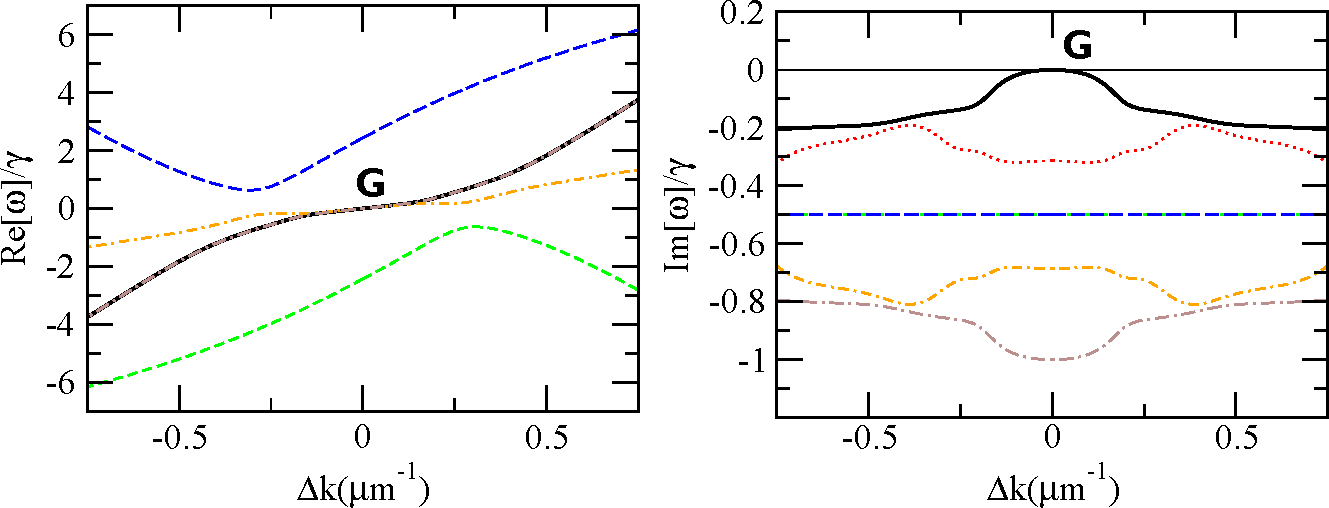
\includegraphics[width=.9\linewidth]{response-ev}
  \caption{
    % 
    Real (left) and imaginary (right) parts of the Bogoliubov spectrum of collective excitations on top of the OPO stationary state as a function of $\Delta k = k - k_{s,p,i}$. The chosen pump intensity is marked with a dotted line in Fig.~\ref{fig:spi}. The breaking of the $U(1)$ symmetry corresponding to the simultaneous phase rotation of the signal and idler is manifest in the presence of the Goldstone mode \textbf{G} (solid heavy curve). From Ref.~\cite{Wouters_2007}.
    % 
  }\label{fig:goldstone}
\end{figure}
% 
Note that both the real and imaginary parts of the frequency of this
gapless mode tend to zero in the long wavelength limit
$\Delta k \rightarrow 0$. Close to this point, the real part has a
non-zero slope due to the finite wavevector of the injected pump
polaritons, while the imaginary part has a parabolic shape. This means
that, as opposed to the BEC case, a localized perturbation in the OPO
regime does not freely propagate as a sound wave. Instead, one should
observe a diffusive-like behaviour, where the localized signal-idler
phase perturbation decays and is then dragged along by the flow of the
pump. Another important difference compared to the BEC spectrum is the
absence of a singularity of the Goldstone branch around the
$\Delta k = 0$ point.

Further insight into OPO physics for realistic experimental conditions
can be gained by numerically solving the full 2-component GP equation
for the coupled exciton and cavity photon fields, as first done in
Ref.~\cite{Whittaker_2005}.  A similar approach, reviewed in detail in
Ref.~\cite{9783642241857}, will be employed in Chapter~\ref{cha:opo},
where we study multicomponent superfluidity in the OPO regime.
%
\begin{figure}[tb]\centering
  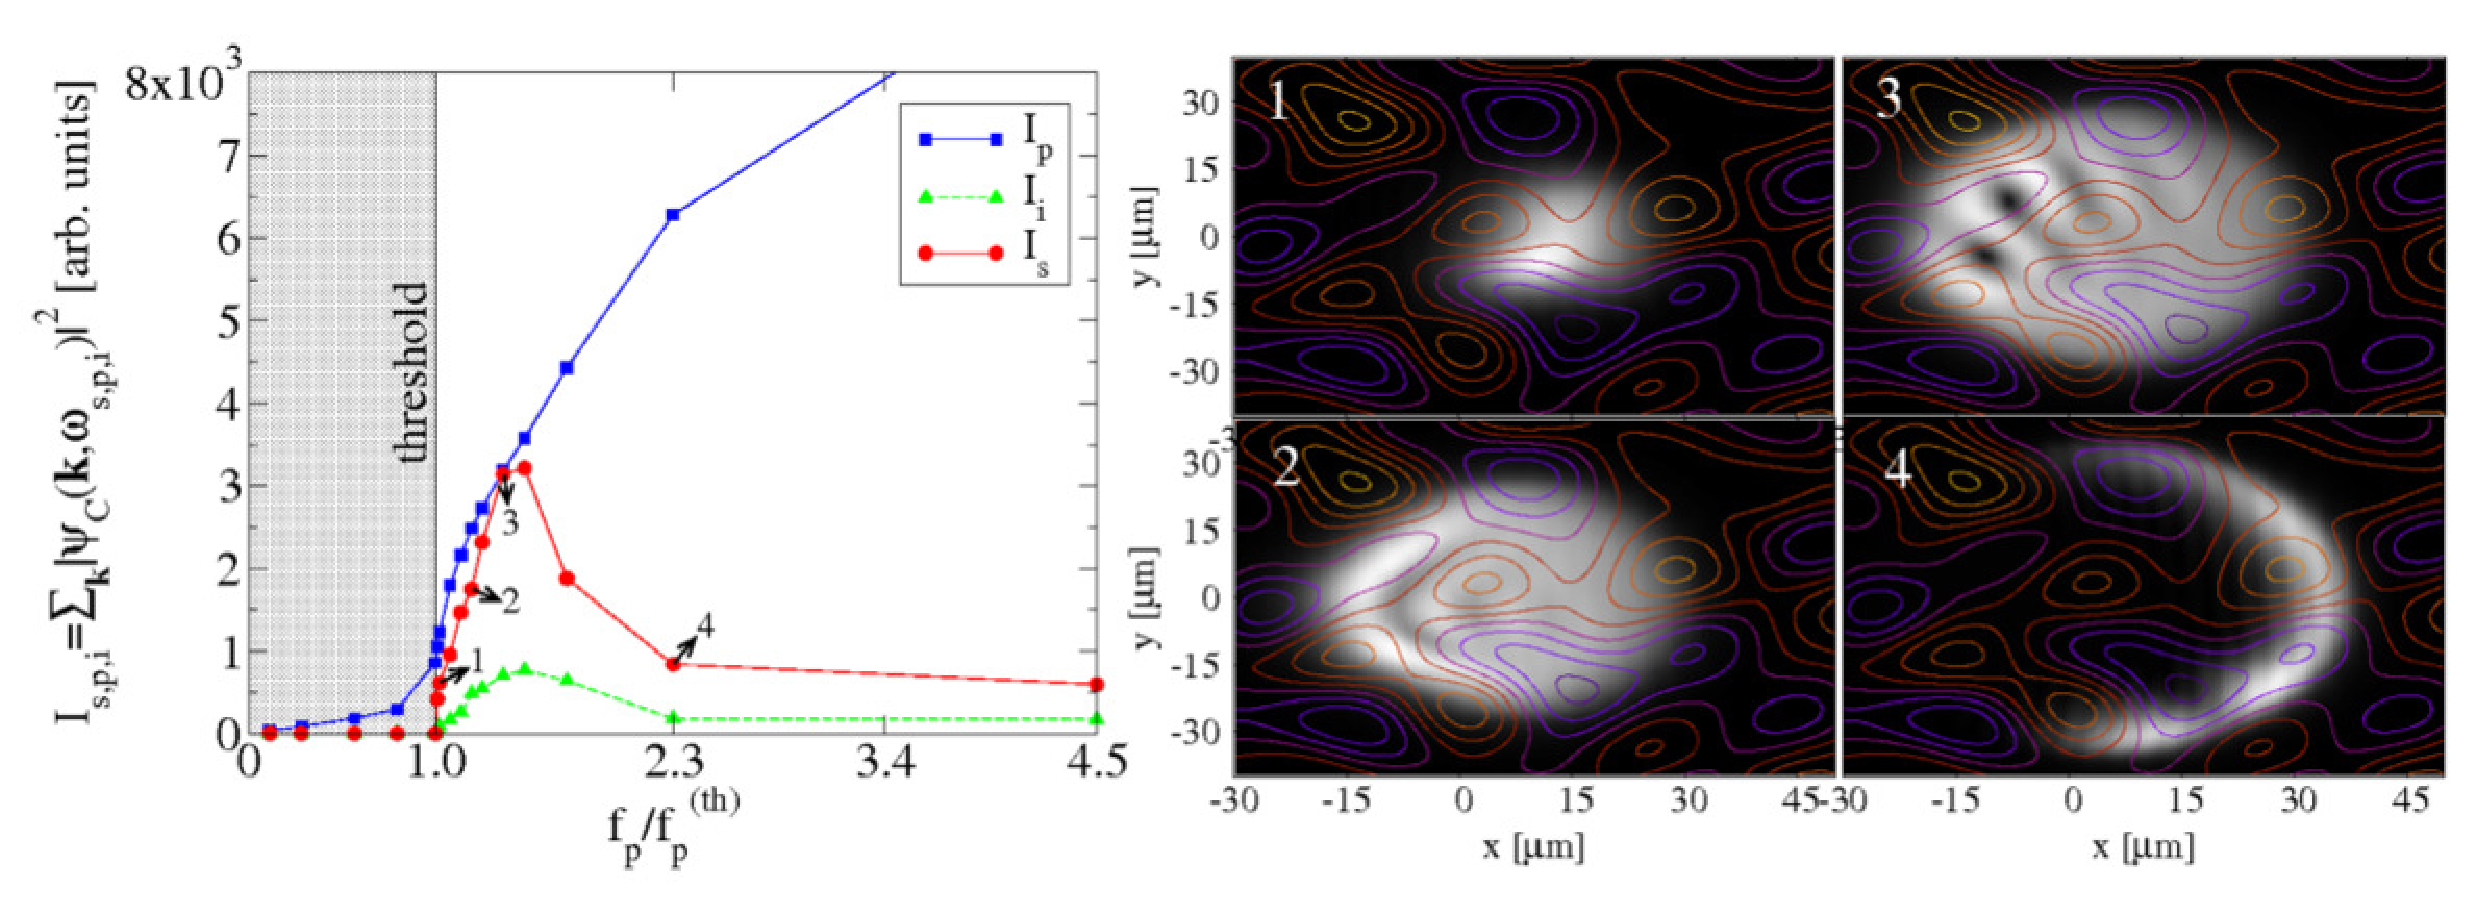
\includegraphics[width=.9\linewidth]{marchetti_threshold_comp}
  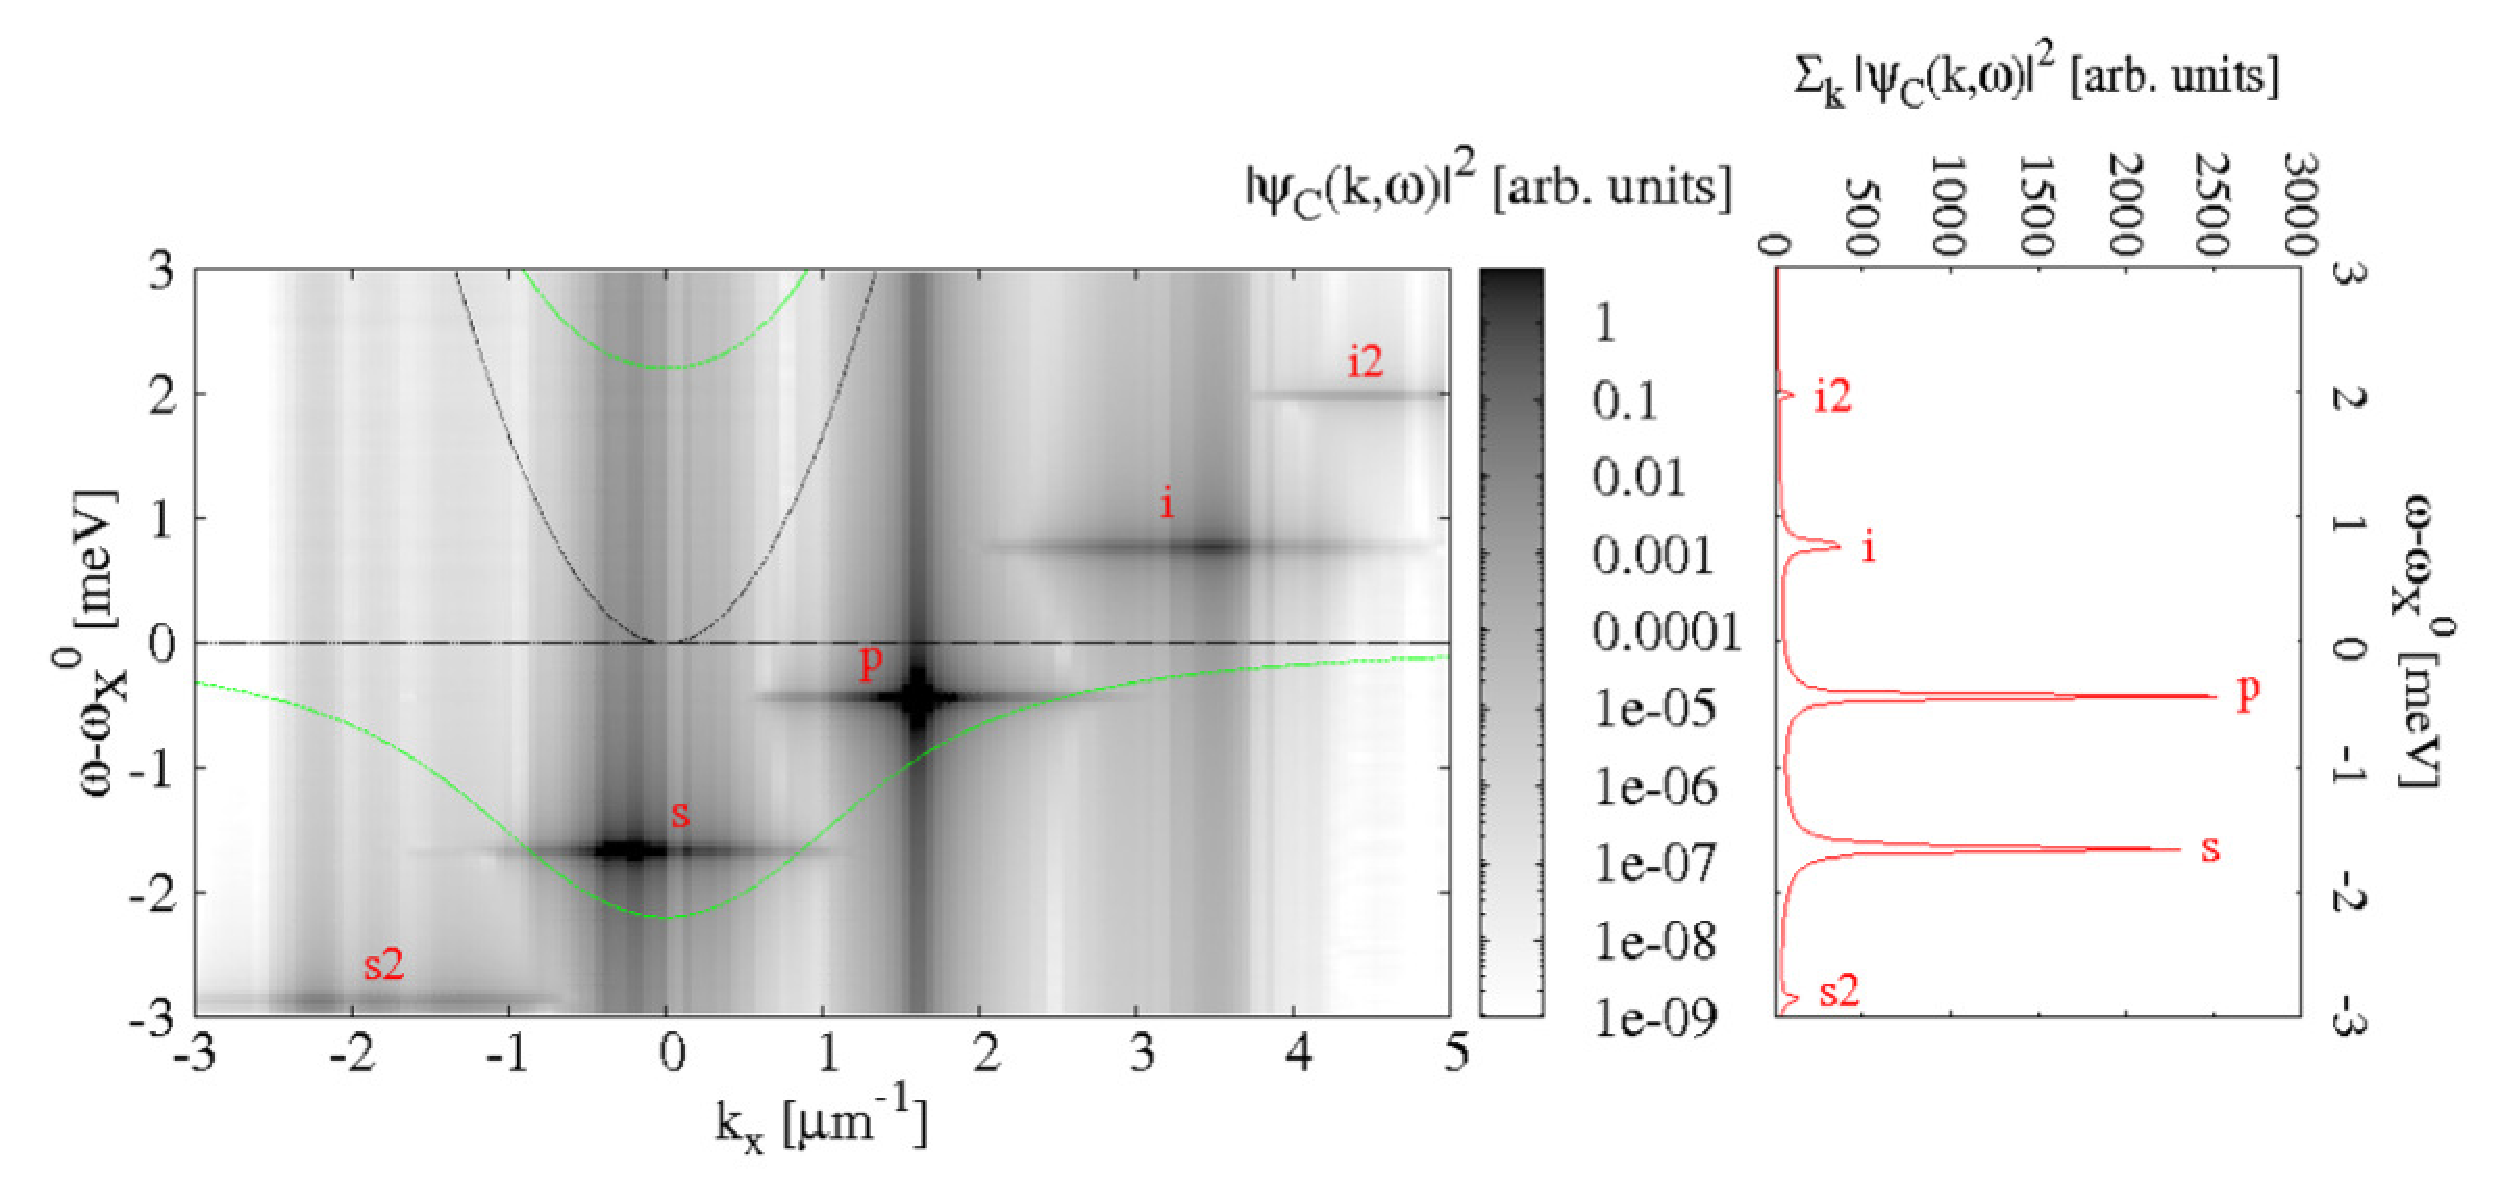
\includegraphics[width=.9\linewidth]{marchetti_spectrum_comp_review}
  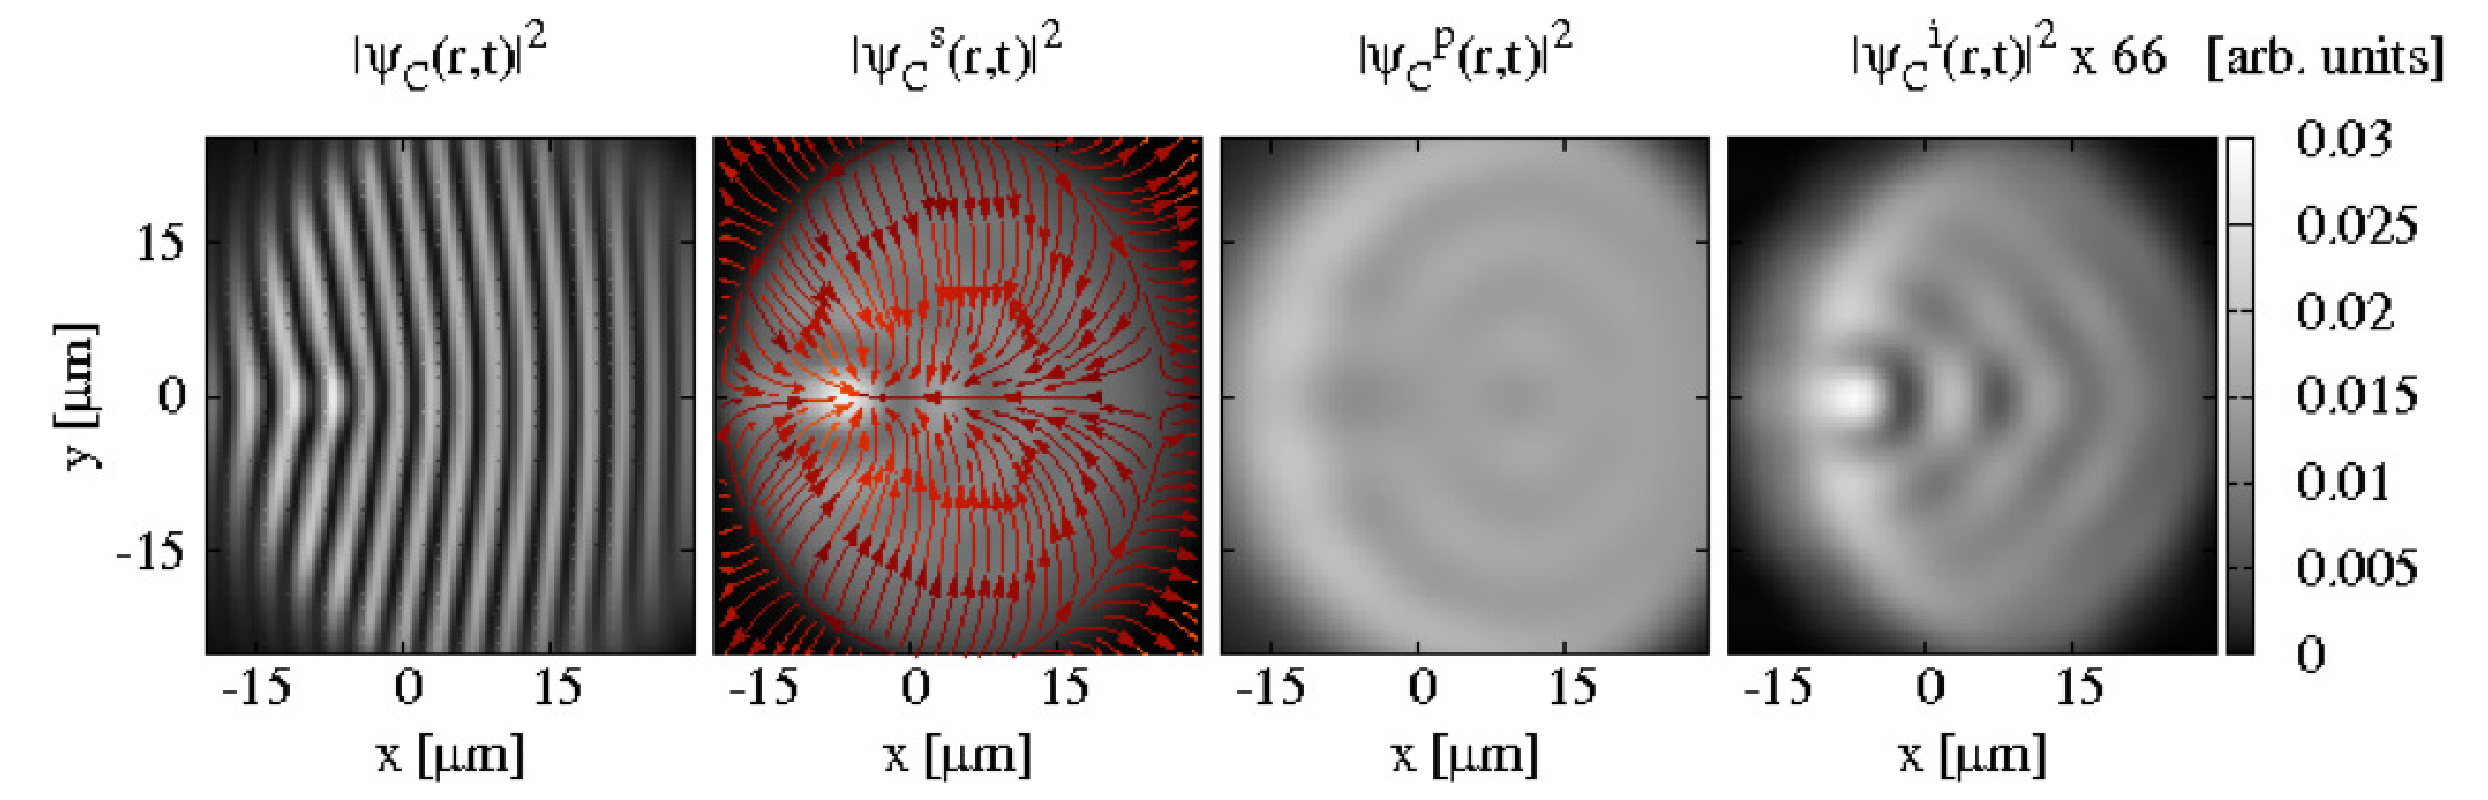
\includegraphics[width=.9\linewidth]{marchetti_comp_OPO_figure_review_clean}
  \caption{
    %
    \emph{Top panels:} Integrated photon emission intensities for the signal $s$ (red dots), pump $p$ (blue squares) and idler $i$ (green triangles) as a function of the renormalized pump intensity (left) and real-space signal emission corresponding to positions 1-4, including random photonic disorder, shown as contour lines (right). Note the OPO phase transition is a gradual one, with the signal first switching on in the center, increasing to maximum size and finally switching off for large pump intensities.
    \emph{Middle panels:} Photonic component of the OPO spectrum (log scale) as a function of energy and momentum (left) and integrated in momentum (right). Note that the emission is $\delta$-like in energy.
    \emph{Bottom panels:} Full photonic emission (left) and filtered real-space emission of signal, pump and idler (last 3 panels). Note the vertical interference fringes caused by the coherent superposition of the 3 states. The arrows in the second panel indicate the complex currents due to  finite size effects.
    From Ref.~\cite{9783642241857}.
    % 
  }\label{fig:marchetti}
\end{figure}
%
Using a continuous wave pump with a top-hat profile, one injects
polaritons at a specific wavevector, close to the inflection point of
the LP dispersion. Above a certain threshold pump power, random
numerical noise starts getting amplified and the OPO instability sets
in, populating the three states. After the system reaches a steady
state, one can obtain the time evolution of the photon and exciton
fields $\psi_C$ and $\psi_X$ both in real and momentum space. Since
experiments measure the photonic component of the polariton field,
that is what is plotted in Fig.~\ref{fig:marchetti}. Filtering in a
narrow cone in momentum (or equivalently, in energy), one can obtain
separately the emission of the signal, pump and idler states, while
the energy-momentum spectrum can be calculated as the discrete Fourier
transform of the total photonic wavefunction recorded at equally
spaced time-intervals.

Inspecting Fig.~\ref{fig:marchetti}, we see that the threshold is a
continuous one in this case, with the OPO first switching on in a
narrow region in the center of the system and then extending to the
size of the whole pump spot before finally surviving only on its edge
when pumping is increased even further. Interestingly, the OPO
transition is signaled by the appearance of a moving striped pattern
in the polariton density (see bottom left panel), spontaneously
breaking the translational symmetry of the system. This pattern is
caused by the interference of the coherent emission of the three
states, and is similar to the Rayleigh-B\'{e}nard instability in the
field of fluid dynamics. The threshold point in the OPO case is where
the stimulated scattering rate exceeds the losses, while the
B\'{e}nard cells form when the temperature gradient (playing the role
of pumping) exceeds the viscosity (dissipation). In these simulations,
the pump (and hence also signal and idler) wavevectors are oriented
along the $\hat{x}$ direction, so the fringes appear along the
$\hat{y}$ axis. They are however usually not visible, due to the time
integration of the photonic emission in most experimental setups. Seen
in this new light, the OPO phase transition has an associated
Goldstone mode that would correspond to a rigid translation of the
spatial stripe pattern.

The photonic component of the OPO spectrum is shown in the middle
pannel of Fig.~\ref{fig:marchetti}. Integrating the spectrum over all
momenta, one sees that, as a result of being in the steady state, the
emission is $\delta$-like in energy, while it is broadened in momentum
due to the finite size of the pump. The satellite states, equally
spaced in energy and less populated, are also visible in the middle
left panel. They are due to secondary scattering processes, from the
signal/idler into the pump and secondary-signal/secondary-idler, and
so on.

Finally, the filtered emission from the signal, pump and idler states
is shown in the lower panels of Fig.~\ref{fig:marchetti}. Since we are
in the steady state, the density profiles are time-independent and
the idler emission is less intense due to the smaller radiative decay
of polaritons at large momenta. One important difference from cold
atomic gases in the BEC regime is the presence of nonvanishing
currents, which can flow across the microcavity even in the ground
state in a polariton system. These currents can be seen in the second
panel for the signal state, and are due the complex interaction
between nonlinearities, dissipation and parametric gain. Note that we
are not refering here to the uniform flow caused by the signal being
at finite momentum $\kv_s$, as in fact this dominant current is
substracted from the plot.


%%% Local Variables:
%%% mode: latex
%%% TeX-master: "../thesis_berceanu"
%%% End:
